\documentclass[1p]{elsarticle_modified}
%\bibliographystyle{elsarticle-num}

%\usepackage[colorlinks]{hyperref}
%\usepackage{abbrmath_seonhwa} %\Abb, \Ascr, \Acal ,\Abf, \Afrak
\usepackage{amsfonts}
\usepackage{amssymb}
\usepackage{amsmath}
\usepackage{amsthm}
\usepackage{scalefnt}
\usepackage{amsbsy}
\usepackage{kotex}
\usepackage{caption}
\usepackage{subfig}
\usepackage{color}
\usepackage{graphicx}
\usepackage{xcolor} %% white, black, red, green, blue, cyan, magenta, yellow
\usepackage{float}
\usepackage{setspace}
\usepackage{hyperref}

\usepackage{tikz}
\usetikzlibrary{arrows}

\usepackage{multirow}
\usepackage{array} % fixed length table
\usepackage{hhline}

%%%%%%%%%%%%%%%%%%%%%
\makeatletter
\renewcommand*\env@matrix[1][\arraystretch]{%
	\edef\arraystretch{#1}%
	\hskip -\arraycolsep
	\let\@ifnextchar\new@ifnextchar
	\array{*\c@MaxMatrixCols c}}
\makeatother %https://tex.stackexchange.com/questions/14071/how-can-i-increase-the-line-spacing-in-a-matrix
%%%%%%%%%%%%%%%

\usepackage[normalem]{ulem}

\newcommand{\msout}[1]{\ifmmode\text{\sout{\ensuremath{#1}}}\else\sout{#1}\fi}
%SOURCE: \msout is \stkout macro in https://tex.stackexchange.com/questions/20609/strikeout-in-math-mode

\newcommand{\cancel}[1]{
	\ifmmode
	{\color{red}\msout{#1}}
	\else
	{\color{red}\sout{#1}}
	\fi
}

\newcommand{\add}[1]{
	{\color{blue}\uwave{#1}}
}

\newcommand{\replace}[2]{
	\ifmmode
	{\color{red}\msout{#1}}{\color{blue}\uwave{#2}}
	\else
	{\color{red}\sout{#1}}{\color{blue}\uwave{#2}}
	\fi
}

\newcommand{\Sol}{\mathcal{S}} %segment
\newcommand{\D}{D} %diagram
\newcommand{\A}{\mathcal{A}} %arc


%%%%%%%%%%%%%%%%%%%%%%%%%%%%%5 test

\def\sl{\operatorname{\textup{SL}}(2,\Cbb)}
\def\psl{\operatorname{\textup{PSL}}(2,\Cbb)}
\def\quan{\mkern 1mu \triangleright \mkern 1mu}

\theoremstyle{definition}
\newtheorem{thm}{Theorem}[section]
\newtheorem{prop}[thm]{Proposition}
\newtheorem{lem}[thm]{Lemma}
\newtheorem{ques}[thm]{Question}
\newtheorem{cor}[thm]{Corollary}
\newtheorem{defn}[thm]{Definition}
\newtheorem{exam}[thm]{Example}
\newtheorem{rmk}[thm]{Remark}
\newtheorem{alg}[thm]{Algorithm}

\newcommand{\I}{\sqrt{-1}}
\begin{document}

%\begin{frontmatter}
%
%\title{Boundary parabolic representations of knots up to 8 crossings}
%
%%% Group authors per affiliation:
%\author{Yunhi Cho} 
%\address{Department of Mathematics, University of Seoul, Seoul, Korea}
%\ead{yhcho@uos.ac.kr}
%
%
%\author{Seonhwa Kim} %\fnref{s_kim}}
%\address{Center for Geometry and Physics, Institute for Basic Science, Pohang, 37673, Korea}
%\ead{ryeona17@ibs.re.kr}
%
%\author{Hyuk Kim}
%\address{Department of Mathematical Sciences, Seoul National University, Seoul 08826, Korea}
%\ead{hyukkim@snu.ac.kr}
%
%\author{Seokbeom Yoon}
%\address{Department of Mathematical Sciences, Seoul National University, Seoul, 08826,  Korea}
%\ead{sbyoon15@snu.ac.kr}
%
%\begin{abstract}
%We find all boundary parabolic representation of knots up to 8 crossings.
%
%\end{abstract}
%\begin{keyword}
%    \MSC[2010] 57M25 
%\end{keyword}
%
%\end{frontmatter}

%\linenumbers
%\tableofcontents
%
\newcommand\colored[1]{\textcolor{white}{\rule[-0.35ex]{0.8em}{1.4ex}}\kern-0.8em\color{red} #1}%
%\newcommand\colored[1]{\textcolor{white}{ #1}\kern-2.17ex	\textcolor{white}{ #1}\kern-1.81ex	\textcolor{white}{ #1}\kern-2.15ex\color{red}#1	}

{\Large $\underline{12a_{1050}~(K12a_{1050})}$}

\setlength{\tabcolsep}{10pt}
\renewcommand{\arraystretch}{1.6}
\vspace{1cm}\begin{tabular}{m{100pt}>{\centering\arraybackslash}m{274pt}}
\multirow{5}{120pt}{
	\centering
	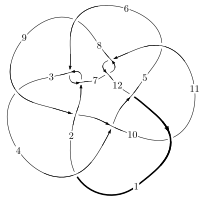
\includegraphics[width=112pt]{../../../GIT/diagram.site/Diagrams/png/1851_12a_1050.png}\\
\ \ \ A knot diagram\footnotemark}&
\allowdisplaybreaks
\textbf{Linearized knot diagam} \\
\cline{2-2}
 &
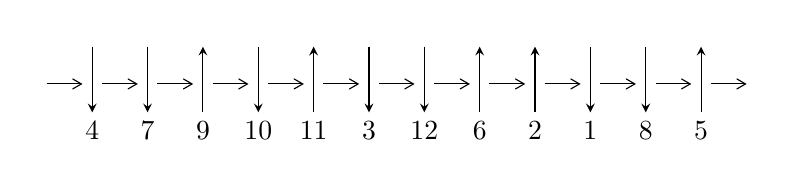
\begin{tikzpicture}[x=20pt, y=17pt]
	% nodes
	\node (C0) at (0, 0) {};
	\node (C1) at (1, 0) {};
	\node (C1U) at (1, +1) {};
	\node (C1D) at (1, -1) {4};

	\node (C2) at (2, 0) {};
	\node (C2U) at (2, +1) {};
	\node (C2D) at (2, -1) {7};

	\node (C3) at (3, 0) {};
	\node (C3U) at (3, +1) {};
	\node (C3D) at (3, -1) {9};

	\node (C4) at (4, 0) {};
	\node (C4U) at (4, +1) {};
	\node (C4D) at (4, -1) {10};

	\node (C5) at (5, 0) {};
	\node (C5U) at (5, +1) {};
	\node (C5D) at (5, -1) {11};

	\node (C6) at (6, 0) {};
	\node (C6U) at (6, +1) {};
	\node (C6D) at (6, -1) {3};

	\node (C7) at (7, 0) {};
	\node (C7U) at (7, +1) {};
	\node (C7D) at (7, -1) {12};

	\node (C8) at (8, 0) {};
	\node (C8U) at (8, +1) {};
	\node (C8D) at (8, -1) {6};

	\node (C9) at (9, 0) {};
	\node (C9U) at (9, +1) {};
	\node (C9D) at (9, -1) {2};

	\node (C10) at (10, 0) {};
	\node (C10U) at (10, +1) {};
	\node (C10D) at (10, -1) {1};

	\node (C11) at (11, 0) {};
	\node (C11U) at (11, +1) {};
	\node (C11D) at (11, -1) {8};

	\node (C12) at (12, 0) {};
	\node (C12U) at (12, +1) {};
	\node (C12D) at (12, -1) {5};
	\node (C13) at (13, 0) {};

	% arrows
	\draw[->,>={angle 60}]
	(C0) edge (C1) (C1) edge (C2) (C2) edge (C3) (C3) edge (C4) (C4) edge (C5) (C5) edge (C6) (C6) edge (C7) (C7) edge (C8) (C8) edge (C9) (C9) edge (C10) (C10) edge (C11) (C11) edge (C12) (C12) edge (C13) ;	\draw[->,>=stealth]
	(C1U) edge (C1D) (C2U) edge (C2D) (C3D) edge (C3U) (C4U) edge (C4D) (C5D) edge (C5U) (C6U) edge (C6D) (C7U) edge (C7D) (C8D) edge (C8U) (C9D) edge (C9U) (C10U) edge (C10D) (C11U) edge (C11D) (C12D) edge (C12U) ;
	\end{tikzpicture} \\
\hhline{~~} \\& 
\textbf{Solving Sequence} \\ \cline{2-2} 
 &
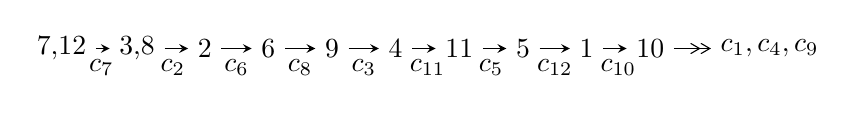
\begin{tikzpicture}[x=23pt, y=7pt]
	% node
	\node (A0) at (-1/8, 0) {7,12};
	\node (A1) at (17/16, 0) {3,8};
	\node (A2) at (17/8, 0) {2};
	\node (A3) at (25/8, 0) {6};
	\node (A4) at (33/8, 0) {9};
	\node (A5) at (41/8, 0) {4};
	\node (A6) at (49/8, 0) {11};
	\node (A7) at (57/8, 0) {5};
	\node (A8) at (65/8, 0) {1};
	\node (A9) at (73/8, 0) {10};
	\node (C1) at (1/2, -1) {$c_{7}$};
	\node (C2) at (13/8, -1) {$c_{2}$};
	\node (C3) at (21/8, -1) {$c_{6}$};
	\node (C4) at (29/8, -1) {$c_{8}$};
	\node (C5) at (37/8, -1) {$c_{3}$};
	\node (C6) at (45/8, -1) {$c_{11}$};
	\node (C7) at (53/8, -1) {$c_{5}$};
	\node (C8) at (61/8, -1) {$c_{12}$};
	\node (C9) at (69/8, -1) {$c_{10}$};
	\node (A10) at (11, 0) {$c_{1},c_{4},c_{9}$};

	% edge
	\draw[->,>=stealth]	
	(A0) edge (A1) (A1) edge (A2) (A2) edge (A3) (A3) edge (A4) (A4) edge (A5) (A5) edge (A6) (A6) edge (A7) (A7) edge (A8) (A8) edge (A9) ;
	\draw[->>,>={angle 60}]	
	(A9) edge (A10);
\end{tikzpicture} \\ 

\end{tabular} \\

\footnotetext{
The image of knot diagram is generated by the software ``\textbf{Draw programme}" developed by Andrew Bartholomew(\url{http://www.layer8.co.uk/maths/draw/index.htm\#Running-draw}), where we modified some parts for our purpose(\url{https://github.com/CATsTAILs/LinksPainter}).
}\phantom \\ \newline 
\centering \textbf{Ideals for irreducible components\footnotemark of $X_{\text{par}}$} 
 
\begin{align*}
I^u_{1}&=\langle 
b- u,\\
\phantom{I^u_{1}}&\phantom{= \langle  }1038287630242143 u^{29}-958498975405341 u^{28}+\cdots+319885682890594 a-1073606987003145,\\
\phantom{I^u_{1}}&\phantom{= \langle  }u^{30}+9 u^{28}+\cdots+u+1\rangle \\
I^u_{2}&=\langle 
-1.41328\times10^{1030} u^{161}-6.25485\times10^{1030} u^{160}+\cdots+1.10537\times10^{1032} b+2.26405\times10^{1037},\\
\phantom{I^u_{2}}&\phantom{= \langle  }-1.18364\times10^{1037} u^{161}-1.15080\times10^{1037} u^{160}+\cdots+5.49710\times10^{1038} a-7.94857\times10^{1043},\\
\phantom{I^u_{2}}&\phantom{= \langle  }u^{162}+2 u^{161}+\cdots-47832405 u-4973081\rangle \\
I^u_{3}&=\langle 
b+u,\;-734 u^{15}+181 u^{14}+\cdots+293 a-1410,\\
\phantom{I^u_{3}}&\phantom{= \langle  }u^{16}+u^{15}+3 u^{14}+2 u^{13}+u^{12}+2 u^{11}-9 u^{10}- u^9-21 u^8-4 u^7-26 u^6-5 u^5-18 u^4-3 u^3-7 u^2- u-1\rangle \\
I^u_{4}&=\langle 
-1.89209\times10^{23} u^{35}-2.03575\times10^{23} u^{34}+\cdots+4.01297\times10^{22} b+1.58103\times10^{23},\\
\phantom{I^u_{4}}&\phantom{= \langle  }-5.17931\times10^{23} u^{35}-1.18836\times10^{24} u^{34}+\cdots+4.01297\times10^{22} a-1.89759\times10^{24},\;u^{36}+u^{35}+\cdots-5 u+1\rangle \\
I^u_{5}&=\langle 
b- u,\;a+2 u-2,\;u^2- u+1\rangle \\
\\
\end{align*}
\raggedright * 5 irreducible components of $\dim_{\mathbb{C}}=0$, with total 246 representations.\\
\footnotetext{All coefficients of polynomials are rational numbers. But the coefficients are sometimes approximated in decimal forms when there is not enough margin.}
\newpage
\renewcommand{\arraystretch}{1}
\centering \section*{I. $I^u_{1}= \langle b- u,\;1.04\times10^{15} u^{29}-9.58\times10^{14} u^{28}+\cdots+3.20\times10^{14} a-1.07\times10^{15},\;u^{30}+9 u^{28}+\cdots+u+1 \rangle$}
\flushleft \textbf{(i) Arc colorings}\\
\begin{tabular}{m{7pt} m{180pt} m{7pt} m{180pt} }
\flushright $a_{7}=$&$\begin{pmatrix}1\\0\end{pmatrix}$ \\
\flushright $a_{12}=$&$\begin{pmatrix}0\\u\end{pmatrix}$ \\
\flushright $a_{3}=$&$\begin{pmatrix}-3.24581 u^{29}+2.99638 u^{28}+\cdots+0.0490322 u+3.35622\\u\end{pmatrix}$ \\
\flushright $a_{8}=$&$\begin{pmatrix}1\\u^2\end{pmatrix}$ \\
\flushright $a_{2}=$&$\begin{pmatrix}-3.24581 u^{29}+2.99638 u^{28}+\cdots+1.04903 u+3.35622\\u\end{pmatrix}$ \\
\flushright $a_{6}=$&$\begin{pmatrix}-2.99638 u^{29}-1.59260 u^{28}+\cdots-6.60203 u-2.24581\\- u^2\end{pmatrix}$ \\
\flushright $a_{9}=$&$\begin{pmatrix}-2.24792 u^{29}+0.435669 u^{28}+\cdots-1.11933 u+1.58988\\0.494712 u^{29}+0.504033 u^{28}+\cdots+2.28664 u+1.07932\end{pmatrix}$ \\
\flushright $a_{4}=$&$\begin{pmatrix}-2.65873 u^{29}+1.54575 u^{28}+\cdots-3.82666 u-0.511097\\0.859974 u^{29}+0.408482 u^{28}+\cdots+1.56275 u+0.0318001\end{pmatrix}$ \\
\flushright $a_{11}=$&$\begin{pmatrix}u\\u^3+u\end{pmatrix}$ \\
\flushright $a_{5}=$&$\begin{pmatrix}-2.28377 u^{29}-1.01732 u^{28}+\cdots-4.29969 u-1.73253\\0.380987 u^{29}+0.209763 u^{28}+\cdots+1.01444 u-0.0620043\end{pmatrix}$ \\
\flushright $a_{1}=$&$\begin{pmatrix}0.149967 u^{29}-1.33960 u^{28}+\cdots-1.47705 u-2.31641\\-1.11679 u^{29}+0.869739 u^{28}+\cdots+0.544449 u+0.862712\end{pmatrix}$ \\
\flushright $a_{10}=$&$\begin{pmatrix}2.50317 u^{29}+1.18430 u^{28}+\cdots+7.47794 u+3.74054\\-0.380987 u^{29}-0.209763 u^{28}+\cdots-1.01444 u+0.0620043\end{pmatrix}$\\&\end{tabular}
\flushleft \textbf{(ii) Obstruction class $= -1$}\\~\\
\flushleft \textbf{(iii) Cusp Shapes $= \frac{342774543239619}{159942841445297} u^{29}+\frac{474438880742083}{159942841445297} u^{28}+\cdots+\frac{4794999154726662}{159942841445297} u+\frac{233245930441382}{159942841445297}$}\\~\\
\newpage\renewcommand{\arraystretch}{1}
\flushleft \textbf{(iv) u-Polynomials at the component}\newline \\
\begin{tabular}{m{50pt}|m{274pt}}
Crossings & \hspace{64pt}u-Polynomials at each crossing \\
\hline $$\begin{aligned}c_{1},c_{10}\end{aligned}$$&$\begin{aligned}
&u^{30}-3 u^{29}+\cdots-2 u+1
\end{aligned}$\\
\hline $$\begin{aligned}c_{2},c_{6},c_{7}\\c_{11}\end{aligned}$$&$\begin{aligned}
&u^{30}+9 u^{28}+\cdots- u+1
\end{aligned}$\\
\hline $$\begin{aligned}c_{3},c_{5}\end{aligned}$$&$\begin{aligned}
&u^{30}- u^{29}+\cdots+12 u+11
\end{aligned}$\\
\hline $$\begin{aligned}c_{4}\end{aligned}$$&$\begin{aligned}
&u^{30}-22 u^{29}+\cdots-17664 u+1536
\end{aligned}$\\
\hline $$\begin{aligned}c_{8}\end{aligned}$$&$\begin{aligned}
&u^{30}+19 u^{29}+\cdots+22608 u+2592
\end{aligned}$\\
\hline $$\begin{aligned}c_{9},c_{12}\end{aligned}$$&$\begin{aligned}
&u^{30}- u^{29}+\cdots+11 u^2+2
\end{aligned}$\\
\hline
\end{tabular}\\~\\
\newpage\renewcommand{\arraystretch}{1}
\flushleft \textbf{(v) Riley Polynomials at the component}\newline \\
\begin{tabular}{m{50pt}|m{274pt}}
Crossings & \hspace{64pt}Riley Polynomials at each crossing \\
\hline $$\begin{aligned}c_{1},c_{10}\end{aligned}$$&$\begin{aligned}
&y^{30}+15 y^{29}+\cdots+30 y+1
\end{aligned}$\\
\hline $$\begin{aligned}c_{2},c_{6},c_{7}\\c_{11}\end{aligned}$$&$\begin{aligned}
&y^{30}+18 y^{29}+\cdots+7 y+1
\end{aligned}$\\
\hline $$\begin{aligned}c_{3},c_{5}\end{aligned}$$&$\begin{aligned}
&y^{30}- y^{29}+\cdots+890 y+121
\end{aligned}$\\
\hline $$\begin{aligned}c_{4}\end{aligned}$$&$\begin{aligned}
&y^{30}+8 y^{29}+\cdots+26935296 y+2359296
\end{aligned}$\\
\hline $$\begin{aligned}c_{8}\end{aligned}$$&$\begin{aligned}
&y^{30}-5 y^{29}+\cdots+33737472 y+6718464
\end{aligned}$\\
\hline $$\begin{aligned}c_{9},c_{12}\end{aligned}$$&$\begin{aligned}
&y^{30}-5 y^{29}+\cdots+44 y+4
\end{aligned}$\\
\hline
\end{tabular}\\~\\
\newpage\flushleft \textbf{(vi) Complex Volumes and Cusp Shapes}
$$\begin{array}{c|c|c}  
\text{Solutions to }I^u_{1}& \I (\text{vol} + \sqrt{-1}CS) & \text{Cusp shape}\\
 \hline 
\begin{aligned}
u &= -0.449233 + 0.940800 I \\
a &= -1.042800 + 0.142208 I \\
b &= -0.449233 + 0.940800 I\end{aligned}
 & \phantom{-}1.29911 + 11.91330 I & \phantom{-}1.70103 - 12.86421 I \\ \hline\begin{aligned}
u &= -0.449233 - 0.940800 I \\
a &= -1.042800 - 0.142208 I \\
b &= -0.449233 - 0.940800 I\end{aligned}
 & \phantom{-}1.29911 - 11.91330 I & \phantom{-}1.70103 + 12.86421 I \\ \hline\begin{aligned}
u &= \phantom{-}1.039650 + 0.080672 I \\
a &= \phantom{-}0.988016 - 0.252509 I \\
b &= \phantom{-}1.039650 + 0.080672 I\end{aligned}
 & -0.50635 + 9.09970 I & -2.62952 - 7.49406 I \\ \hline\begin{aligned}
u &= \phantom{-}1.039650 - 0.080672 I \\
a &= \phantom{-}0.988016 + 0.252509 I \\
b &= \phantom{-}1.039650 - 0.080672 I\end{aligned}
 & -0.50635 - 9.09970 I & -2.62952 + 7.49406 I \\ \hline\begin{aligned}
u &= -0.192642 + 0.892017 I \\
a &= -1.116590 - 0.674078 I \\
b &= -0.192642 + 0.892017 I\end{aligned}
 & \phantom{-}3.81522 - 0.95935 I & \phantom{-}6.29739 + 2.72741 I \\ \hline\begin{aligned}
u &= -0.192642 - 0.892017 I \\
a &= -1.116590 + 0.674078 I \\
b &= -0.192642 - 0.892017 I\end{aligned}
 & \phantom{-}3.81522 + 0.95935 I & \phantom{-}6.29739 - 2.72741 I \\ \hline\begin{aligned}
u &= \phantom{-}0.528654 + 0.725501 I \\
a &= \phantom{-}0.207468 - 0.513474 I \\
b &= \phantom{-}0.528654 + 0.725501 I\end{aligned}
 & -1.12796 - 2.16922 I & -4.84782 + 3.12859 I \\ \hline\begin{aligned}
u &= \phantom{-}0.528654 - 0.725501 I \\
a &= \phantom{-}0.207468 + 0.513474 I \\
b &= \phantom{-}0.528654 - 0.725501 I\end{aligned}
 & -1.12796 + 2.16922 I & -4.84782 - 3.12859 I \\ \hline\begin{aligned}
u &= \phantom{-}0.216729 + 1.101220 I \\
a &= \phantom{-}0.12091 - 2.80714 I \\
b &= \phantom{-}0.216729 + 1.101220 I\end{aligned}
 & \phantom{-}4.12713 - 2.60846 I & \phantom{-}4.07410 + 8.65048 I \\ \hline\begin{aligned}
u &= \phantom{-}0.216729 - 1.101220 I \\
a &= \phantom{-}0.12091 + 2.80714 I \\
b &= \phantom{-}0.216729 - 1.101220 I\end{aligned}
 & \phantom{-}4.12713 + 2.60846 I & \phantom{-}4.07410 - 8.65048 I\\
 \hline 
 \end{array}$$\newpage$$\begin{array}{c|c|c}  
\text{Solutions to }I^u_{1}& \I (\text{vol} + \sqrt{-1}CS) & \text{Cusp shape}\\
 \hline 
\begin{aligned}
u &= \phantom{-}0.334146 + 0.806203 I \\
a &= \phantom{-}0.97112 + 1.30413 I \\
b &= \phantom{-}0.334146 + 0.806203 I\end{aligned}
 & \phantom{-}2.39563 - 1.87382 I & \phantom{-}2.69727 + 2.55936 I \\ \hline\begin{aligned}
u &= \phantom{-}0.334146 - 0.806203 I \\
a &= \phantom{-}0.97112 - 1.30413 I \\
b &= \phantom{-}0.334146 - 0.806203 I\end{aligned}
 & \phantom{-}2.39563 + 1.87382 I & \phantom{-}2.69727 - 2.55936 I \\ \hline\begin{aligned}
u &= \phantom{-}0.008350 + 0.766245 I \\
a &= \phantom{-}1.31335 - 4.65457 I \\
b &= \phantom{-}0.008350 + 0.766245 I\end{aligned}
 & -0.91288 - 6.45984 I & \phantom{-}6.96574 + 6.19266 I \\ \hline\begin{aligned}
u &= \phantom{-}0.008350 - 0.766245 I \\
a &= \phantom{-}1.31335 + 4.65457 I \\
b &= \phantom{-}0.008350 - 0.766245 I\end{aligned}
 & -0.91288 + 6.45984 I & \phantom{-}6.96574 - 6.19266 I \\ \hline\begin{aligned}
u &= -0.746790 + 0.129308 I \\
a &= -0.581917 - 0.242711 I \\
b &= -0.746790 + 0.129308 I\end{aligned}
 & \phantom{-}1.94728 - 2.37977 I & \phantom{-}0.01549 + 3.22068 I \\ \hline\begin{aligned}
u &= -0.746790 - 0.129308 I \\
a &= -0.581917 + 0.242711 I \\
b &= -0.746790 - 0.129308 I\end{aligned}
 & \phantom{-}1.94728 + 2.37977 I & \phantom{-}0.01549 - 3.22068 I \\ \hline\begin{aligned}
u &= -0.339807 + 1.223790 I \\
a &= -0.89868 - 2.29972 I \\
b &= -0.339807 + 1.223790 I\end{aligned}
 & \phantom{-}9.08252 + 4.70541 I & \phantom{-}7.58999 - 4.89180 I \\ \hline\begin{aligned}
u &= -0.339807 - 1.223790 I \\
a &= -0.89868 + 2.29972 I \\
b &= -0.339807 - 1.223790 I\end{aligned}
 & \phantom{-}9.08252 - 4.70541 I & \phantom{-}7.58999 + 4.89180 I \\ \hline\begin{aligned}
u &= -0.598923 + 0.180377 I \\
a &= -1.19103 - 2.17009 I \\
b &= -0.598923 + 0.180377 I\end{aligned}
 & -2.84910 + 6.12107 I & -11.6552 - 8.5759 I \\ \hline\begin{aligned}
u &= -0.598923 - 0.180377 I \\
a &= -1.19103 + 2.17009 I \\
b &= -0.598923 - 0.180377 I\end{aligned}
 & -2.84910 - 6.12107 I & -11.6552 + 8.5759 I\\
 \hline 
 \end{array}$$\newpage$$\begin{array}{c|c|c}  
\text{Solutions to }I^u_{1}& \I (\text{vol} + \sqrt{-1}CS) & \text{Cusp shape}\\
 \hline 
\begin{aligned}
u &= -0.545038 + 1.269990 I \\
a &= -1.05931 - 1.88668 I \\
b &= -0.545038 + 1.269990 I\end{aligned}
 & \phantom{-}8.6354 + 12.3602 I & \phantom{-}6.89874 - 8.94538 I \\ \hline\begin{aligned}
u &= -0.545038 - 1.269990 I \\
a &= -1.05931 + 1.88668 I \\
b &= -0.545038 - 1.269990 I\end{aligned}
 & \phantom{-}8.6354 - 12.3602 I & \phantom{-}6.89874 + 8.94538 I \\ \hline\begin{aligned}
u &= -0.76172 + 1.19937 I \\
a &= -1.29587 - 1.18790 I \\
b &= -0.76172 + 1.19937 I\end{aligned}
 & \phantom{-}6.51330 + 6.47115 I & \phantom{-}3.75399 - 6.89218 I \\ \hline\begin{aligned}
u &= -0.76172 - 1.19937 I \\
a &= -1.29587 + 1.18790 I \\
b &= -0.76172 - 1.19937 I\end{aligned}
 & \phantom{-}6.51330 - 6.47115 I & \phantom{-}3.75399 + 6.89218 I \\ \hline\begin{aligned}
u &= \phantom{-}0.313821 + 0.430877 I \\
a &= -0.606847 - 0.536231 I \\
b &= \phantom{-}0.313821 + 0.430877 I\end{aligned}
 & -0.192876 - 1.170060 I & -2.11608 + 6.41291 I \\ \hline\begin{aligned}
u &= \phantom{-}0.313821 - 0.430877 I \\
a &= -0.606847 + 0.536231 I \\
b &= \phantom{-}0.313821 - 0.430877 I\end{aligned}
 & -0.192876 + 1.170060 I & -2.11608 - 6.41291 I \\ \hline\begin{aligned}
u &= \phantom{-}0.66183 + 1.33533 I \\
a &= \phantom{-}1.03587 - 1.54140 I \\
b &= \phantom{-}0.66183 + 1.33533 I\end{aligned}
 & \phantom{-}6.7565 - 21.4337 I & \phantom{-}1.89596 + 10.81516 I \\ \hline\begin{aligned}
u &= \phantom{-}0.66183 - 1.33533 I \\
a &= \phantom{-}1.03587 + 1.54140 I \\
b &= \phantom{-}0.66183 - 1.33533 I\end{aligned}
 & \phantom{-}6.7565 + 21.4337 I & \phantom{-}1.89596 - 10.81516 I \\ \hline\begin{aligned}
u &= \phantom{-}0.53097 + 1.50169 I \\
a &= \phantom{-}0.65631 - 1.42667 I \\
b &= \phantom{-}0.53097 + 1.50169 I\end{aligned}
 & \phantom{-}8.72016 - 3.34746 I & \phantom{-}7.85889 + 0.87317 I \\ \hline\begin{aligned}
u &= \phantom{-}0.53097 - 1.50169 I \\
a &= \phantom{-}0.65631 + 1.42667 I \\
b &= \phantom{-}0.53097 - 1.50169 I\end{aligned}
 & \phantom{-}8.72016 + 3.34746 I & \phantom{-}7.85889 - 0.87317 I\\
 \hline 
 \end{array}$$\newpage\newpage\renewcommand{\arraystretch}{1}
\centering \section*{II. $I^u_{2}= \langle -1.41\times10^{1030} u^{161}-6.25\times10^{1030} u^{160}+\cdots+1.11\times10^{1032} b+2.26\times10^{1037},\;-1.18\times10^{1037} u^{161}-1.15\times10^{1037} u^{160}+\cdots+5.50\times10^{1038} a-7.95\times10^{1043},\;u^{162}+2 u^{161}+\cdots-47832405 u-4973081 \rangle$}
\flushleft \textbf{(i) Arc colorings}\\
\begin{tabular}{m{7pt} m{180pt} m{7pt} m{180pt} }
\flushright $a_{7}=$&$\begin{pmatrix}1\\0\end{pmatrix}$ \\
\flushright $a_{12}=$&$\begin{pmatrix}0\\u\end{pmatrix}$ \\
\flushright $a_{3}=$&$\begin{pmatrix}0.0215320 u^{161}+0.0209347 u^{160}+\cdots+1.26150\times10^{6} u+144596.\\0.0127856 u^{161}+0.0565860 u^{160}+\cdots-2.04836\times10^{6} u-204823.\end{pmatrix}$ \\
\flushright $a_{8}=$&$\begin{pmatrix}1\\u^2\end{pmatrix}$ \\
\flushright $a_{2}=$&$\begin{pmatrix}0.0343177 u^{161}+0.0775207 u^{160}+\cdots-786853. u-60227.2\\0.0127856 u^{161}+0.0565860 u^{160}+\cdots-2.04836\times10^{6} u-204823.\end{pmatrix}$ \\
\flushright $a_{6}=$&$\begin{pmatrix}-0.0211515 u^{161}-0.0906693 u^{160}+\cdots+3.11461\times10^{6} u+310143.\\0.00672843 u^{161}+0.0300770 u^{160}+\cdots-1.19310\times10^{6} u-119473.\end{pmatrix}$ \\
\flushright $a_{9}=$&$\begin{pmatrix}0.0422973 u^{161}+0.0991295 u^{160}+\cdots-1.59305\times10^{6} u-138499.\\0.00681074 u^{161}+0.00910050 u^{160}+\cdots+300382. u+34734.8\end{pmatrix}$ \\
\flushright $a_{4}=$&$\begin{pmatrix}0.0684913 u^{161}+0.264874 u^{160}+\cdots-7.29836\times10^{6} u-718586.\\-0.00950507 u^{161}-0.0170791 u^{160}+\cdots+198269. u+9569.50\end{pmatrix}$ \\
\flushright $a_{11}=$&$\begin{pmatrix}u\\u^3+u\end{pmatrix}$ \\
\flushright $a_{5}=$&$\begin{pmatrix}-0.0126198 u^{161}-0.0530040 u^{160}+\cdots+1.70926\times10^{6} u+169761.\\0.00878790 u^{161}+0.0400472 u^{160}+\cdots-1.57058\times10^{6} u-157399.\end{pmatrix}$ \\
\flushright $a_{1}=$&$\begin{pmatrix}-0.0119242 u^{161}+0.00757900 u^{160}+\cdots-1.69460\times10^{6} u-187863.\\0.0134614 u^{161}+0.0466547 u^{160}+\cdots-1.33051\times10^{6} u-128598.\end{pmatrix}$ \\
\flushright $a_{10}=$&$\begin{pmatrix}0.0578349 u^{161}+0.139788 u^{160}+\cdots-2.13978\times10^{6} u-182492.\\0.0210823 u^{161}+0.0177459 u^{160}+\cdots+1.60534\times10^{6} u+180830.\end{pmatrix}$\\&\end{tabular}
\flushleft \textbf{(ii) Obstruction class $= -1$}\\~\\
\flushleft \textbf{(iii) Cusp Shapes $= 0.128045 u^{161}+0.241674 u^{160}+\cdots+417800. u+122922.$}\\~\\
\newpage\renewcommand{\arraystretch}{1}
\flushleft \textbf{(iv) u-Polynomials at the component}\newline \\
\begin{tabular}{m{50pt}|m{274pt}}
Crossings & \hspace{64pt}u-Polynomials at each crossing \\
\hline $$\begin{aligned}c_{1},c_{10}\end{aligned}$$&$\begin{aligned}
&u^{162}-15 u^{161}+\cdots-1915810 u+78157
\end{aligned}$\\
\hline $$\begin{aligned}c_{2},c_{6},c_{7}\\c_{11}\end{aligned}$$&$\begin{aligned}
&u^{162}-2 u^{161}+\cdots+47832405 u-4973081
\end{aligned}$\\
\hline $$\begin{aligned}c_{3},c_{5}\end{aligned}$$&$\begin{aligned}
&u^{162}-5 u^{161}+\cdots-1263792898 u-135983129
\end{aligned}$\\
\hline $$\begin{aligned}c_{4}\end{aligned}$$&$\begin{aligned}
&(u^{81}+4 u^{80}+\cdots-9 u+1)^{2}
\end{aligned}$\\
\hline $$\begin{aligned}c_{8}\end{aligned}$$&$\begin{aligned}
&(u^{81}-13 u^{80}+\cdots-348250 u-398125)^{2}
\end{aligned}$\\
\hline $$\begin{aligned}c_{9},c_{12}\end{aligned}$$&$\begin{aligned}
&u^{162}-13 u^{161}+\cdots-1252 u+5341
\end{aligned}$\\
\hline
\end{tabular}\\~\\
\newpage\renewcommand{\arraystretch}{1}
\flushleft \textbf{(v) Riley Polynomials at the component}\newline \\
\begin{tabular}{m{50pt}|m{274pt}}
Crossings & \hspace{64pt}Riley Polynomials at each crossing \\
\hline $$\begin{aligned}c_{1},c_{10}\end{aligned}$$&$\begin{aligned}
&y^{162}-5 y^{161}+\cdots+315891474626 y+6108516649
\end{aligned}$\\
\hline $$\begin{aligned}c_{2},c_{6},c_{7}\\c_{11}\end{aligned}$$&$\begin{aligned}
&y^{162}+96 y^{161}+\cdots+1122280033576759 y+24731534632561
\end{aligned}$\\
\hline $$\begin{aligned}c_{3},c_{5}\end{aligned}$$&$\begin{aligned}
&y^{162}-79 y^{161}+\cdots-1050391772674517412 y+18491411372630641
\end{aligned}$\\
\hline $$\begin{aligned}c_{4}\end{aligned}$$&$\begin{aligned}
&(y^{81}-36 y^{80}+\cdots+151 y-1)^{2}
\end{aligned}$\\
\hline $$\begin{aligned}c_{8}\end{aligned}$$&$\begin{aligned}
&(y^{81}-65 y^{80}+\cdots+3852346312500 y-158503515625)^{2}
\end{aligned}$\\
\hline $$\begin{aligned}c_{9},c_{12}\end{aligned}$$&$\begin{aligned}
&y^{162}+29 y^{161}+\cdots-2042438378 y+28526281
\end{aligned}$\\
\hline
\end{tabular}\\~\\
\newpage\flushleft \textbf{(vi) Complex Volumes and Cusp Shapes}
$$\begin{array}{c|c|c}  
\text{Solutions to }I^u_{2}& \I (\text{vol} + \sqrt{-1}CS) & \text{Cusp shape}\\
 \hline 
\begin{aligned}
u &= \phantom{-}0.512433 + 0.858107 I \\
a &= -1.56439 - 1.14376 I \\
b &= -0.021504 - 0.885713 I\end{aligned}
 & \phantom{-}2.62612 - 2.03925 I & \phantom{-0.000000 } 0 \\ \hline\begin{aligned}
u &= \phantom{-}0.512433 - 0.858107 I \\
a &= -1.56439 + 1.14376 I \\
b &= -0.021504 + 0.885713 I\end{aligned}
 & \phantom{-}2.62612 + 2.03925 I & \phantom{-0.000000 } 0 \\ \hline\begin{aligned}
u &= \phantom{-}0.145803 + 0.995620 I \\
a &= -0.12521 + 2.89018 I \\
b &= -0.21774 - 1.48046 I\end{aligned}
 & \phantom{-}4.97164 - 0.41306 I & \phantom{-0.000000 } 0 \\ \hline\begin{aligned}
u &= \phantom{-}0.145803 - 0.995620 I \\
a &= -0.12521 - 2.89018 I \\
b &= -0.21774 + 1.48046 I\end{aligned}
 & \phantom{-}4.97164 + 0.41306 I & \phantom{-0.000000 } 0 \\ \hline\begin{aligned}
u &= \phantom{-}0.757871 + 0.640617 I \\
a &= \phantom{-}0.223968 + 0.318131 I \\
b &= -0.168701 + 1.066500 I\end{aligned}
 & -0.450299 + 0.683300 I & \phantom{-0.000000 } 0 \\ \hline\begin{aligned}
u &= \phantom{-}0.757871 - 0.640617 I \\
a &= \phantom{-}0.223968 - 0.318131 I \\
b &= -0.168701 - 1.066500 I\end{aligned}
 & -0.450299 - 0.683300 I & \phantom{-0.000000 } 0 \\ \hline\begin{aligned}
u &= -0.935488 + 0.378434 I \\
a &= -0.493795 - 0.101544 I \\
b &= -0.291077 + 0.780516 I\end{aligned}
 & -1.21159 - 3.47818 I & \phantom{-0.000000 } 0 \\ \hline\begin{aligned}
u &= -0.935488 - 0.378434 I \\
a &= -0.493795 + 0.101544 I \\
b &= -0.291077 - 0.780516 I\end{aligned}
 & -1.21159 + 3.47818 I & \phantom{-0.000000 } 0 \\ \hline\begin{aligned}
u &= -1.009490 + 0.082758 I \\
a &= \phantom{-}0.144527 - 0.572008 I \\
b &= \phantom{-}0.279301 + 1.280210 I\end{aligned}
 & \phantom{-}5.28165 - 6.21646 I & \phantom{-0.000000 } 0 \\ \hline\begin{aligned}
u &= -1.009490 - 0.082758 I \\
a &= \phantom{-}0.144527 + 0.572008 I \\
b &= \phantom{-}0.279301 - 1.280210 I\end{aligned}
 & \phantom{-}5.28165 + 6.21646 I & \phantom{-0.000000 } 0\\
 \hline 
 \end{array}$$\newpage$$\begin{array}{c|c|c}  
\text{Solutions to }I^u_{2}& \I (\text{vol} + \sqrt{-1}CS) & \text{Cusp shape}\\
 \hline 
\begin{aligned}
u &= \phantom{-}0.412029 + 0.891858 I \\
a &= -0.683993 - 0.241671 I \\
b &= -0.533283 + 0.580692 I\end{aligned}
 & -0.95013 - 2.08177 I & \phantom{-0.000000 } 0 \\ \hline\begin{aligned}
u &= \phantom{-}0.412029 - 0.891858 I \\
a &= -0.683993 + 0.241671 I \\
b &= -0.533283 - 0.580692 I\end{aligned}
 & -0.95013 + 2.08177 I & \phantom{-0.000000 } 0 \\ \hline\begin{aligned}
u &= \phantom{-}0.519713 + 0.810533 I \\
a &= \phantom{-}3.34397 - 1.12815 I \\
b &= \phantom{-}0.067527 - 0.928521 I\end{aligned}
 & \phantom{-}3.14164 - 1.81489 I & \phantom{-0.000000 } 0 \\ \hline\begin{aligned}
u &= \phantom{-}0.519713 - 0.810533 I \\
a &= \phantom{-}3.34397 + 1.12815 I \\
b &= \phantom{-}0.067527 + 0.928521 I\end{aligned}
 & \phantom{-}3.14164 + 1.81489 I & \phantom{-0.000000 } 0 \\ \hline\begin{aligned}
u &= -0.955469 + 0.100910 I \\
a &= -0.526877 + 0.609433 I \\
b &= -0.480389 - 1.194020 I\end{aligned}
 & \phantom{-}5.08464 - 6.96702 I & \phantom{-0.000000 } 0 \\ \hline\begin{aligned}
u &= -0.955469 - 0.100910 I \\
a &= -0.526877 - 0.609433 I \\
b &= -0.480389 + 1.194020 I\end{aligned}
 & \phantom{-}5.08464 + 6.96702 I & \phantom{-0.000000 } 0 \\ \hline\begin{aligned}
u &= \phantom{-}0.111590 + 1.053510 I \\
a &= -0.17695 + 2.23642 I \\
b &= -0.85395 - 1.30740 I\end{aligned}
 & \phantom{-}5.44010 - 4.01731 I & \phantom{-0.000000 } 0 \\ \hline\begin{aligned}
u &= \phantom{-}0.111590 - 1.053510 I \\
a &= -0.17695 - 2.23642 I \\
b &= -0.85395 + 1.30740 I\end{aligned}
 & \phantom{-}5.44010 + 4.01731 I & \phantom{-0.000000 } 0 \\ \hline\begin{aligned}
u &= -0.209883 + 0.916511 I \\
a &= -0.936561 + 0.160907 I \\
b &= \phantom{-}1.047010 + 0.532708 I\end{aligned}
 & -1.156040 - 0.497979 I & \phantom{-0.000000 } 0 \\ \hline\begin{aligned}
u &= -0.209883 - 0.916511 I \\
a &= -0.936561 - 0.160907 I \\
b &= \phantom{-}1.047010 - 0.532708 I\end{aligned}
 & -1.156040 + 0.497979 I & \phantom{-0.000000 } 0\\
 \hline 
 \end{array}$$\newpage$$\begin{array}{c|c|c}  
\text{Solutions to }I^u_{2}& \I (\text{vol} + \sqrt{-1}CS) & \text{Cusp shape}\\
 \hline 
\begin{aligned}
u &= -0.203861 + 1.047750 I \\
a &= -1.131320 + 0.390938 I \\
b &= -0.596978 - 0.695658 I\end{aligned}
 & \phantom{-}0.55788 + 7.73645 I & \phantom{-0.000000 } 0 \\ \hline\begin{aligned}
u &= -0.203861 - 1.047750 I \\
a &= -1.131320 - 0.390938 I \\
b &= -0.596978 + 0.695658 I\end{aligned}
 & \phantom{-}0.55788 - 7.73645 I & \phantom{-0.000000 } 0 \\ \hline\begin{aligned}
u &= \phantom{-}0.067527 + 0.928521 I \\
a &= -2.06891 - 3.00695 I \\
b &= \phantom{-}0.519713 - 0.810533 I\end{aligned}
 & \phantom{-}3.14164 + 1.81489 I & \phantom{-0.000000 } 0 \\ \hline\begin{aligned}
u &= \phantom{-}0.067527 - 0.928521 I \\
a &= -2.06891 + 3.00695 I \\
b &= \phantom{-}0.519713 + 0.810533 I\end{aligned}
 & \phantom{-}3.14164 - 1.81489 I & \phantom{-0.000000 } 0 \\ \hline\begin{aligned}
u &= -0.403847 + 1.001040 I \\
a &= \phantom{-}0.972188 + 0.638285 I \\
b &= \phantom{-}0.638989 - 0.893575 I\end{aligned}
 & \phantom{-}0.29347 + 5.89699 I & \phantom{-0.000000 } 0 \\ \hline\begin{aligned}
u &= -0.403847 - 1.001040 I \\
a &= \phantom{-}0.972188 - 0.638285 I \\
b &= \phantom{-}0.638989 + 0.893575 I\end{aligned}
 & \phantom{-}0.29347 - 5.89699 I & \phantom{-0.000000 } 0 \\ \hline\begin{aligned}
u &= -0.168701 + 1.066500 I \\
a &= \phantom{-}0.356727 - 0.024490 I \\
b &= \phantom{-}0.757871 + 0.640617 I\end{aligned}
 & -0.450299 + 0.683300 I & \phantom{-0.000000 } 0 \\ \hline\begin{aligned}
u &= -0.168701 - 1.066500 I \\
a &= \phantom{-}0.356727 + 0.024490 I \\
b &= \phantom{-}0.757871 - 0.640617 I\end{aligned}
 & -0.450299 - 0.683300 I & \phantom{-0.000000 } 0 \\ \hline\begin{aligned}
u &= -0.596978 + 0.695658 I \\
a &= \phantom{-}1.174400 - 0.750538 I \\
b &= -0.203861 - 1.047750 I\end{aligned}
 & \phantom{-}0.55788 - 7.73645 I & \phantom{-0.000000 } 0 \\ \hline\begin{aligned}
u &= -0.596978 - 0.695658 I \\
a &= \phantom{-}1.174400 + 0.750538 I \\
b &= -0.203861 + 1.047750 I\end{aligned}
 & \phantom{-}0.55788 + 7.73645 I & \phantom{-0.000000 } 0\\
 \hline 
 \end{array}$$\newpage$$\begin{array}{c|c|c}  
\text{Solutions to }I^u_{2}& \I (\text{vol} + \sqrt{-1}CS) & \text{Cusp shape}\\
 \hline 
\begin{aligned}
u &= \phantom{-}0.556675 + 0.721239 I \\
a &= -0.486203 + 0.128189 I \\
b &= \phantom{-}0.470448 - 0.329063 I\end{aligned}
 & -1.18885 - 2.26631 I & \phantom{-0.000000 } 0 \\ \hline\begin{aligned}
u &= \phantom{-}0.556675 - 0.721239 I \\
a &= -0.486203 - 0.128189 I \\
b &= \phantom{-}0.470448 + 0.329063 I\end{aligned}
 & -1.18885 + 2.26631 I & \phantom{-0.000000 } 0 \\ \hline\begin{aligned}
u &= -0.307643 + 1.045480 I \\
a &= -0.71470 - 2.54306 I \\
b &= -0.56943 + 1.36887 I\end{aligned}
 & \phantom{-}2.87307 + 11.89210 I & \phantom{-0.000000 } 0 \\ \hline\begin{aligned}
u &= -0.307643 - 1.045480 I \\
a &= -0.71470 + 2.54306 I \\
b &= -0.56943 - 1.36887 I\end{aligned}
 & \phantom{-}2.87307 - 11.89210 I & \phantom{-0.000000 } 0 \\ \hline\begin{aligned}
u &= \phantom{-}0.108889 + 1.086580 I \\
a &= \phantom{-}0.37526 - 3.67069 I \\
b &= \phantom{-}0.453686 + 1.003950 I\end{aligned}
 & \phantom{-}3.76566 - 2.19626 I & \phantom{-0.000000 } 0 \\ \hline\begin{aligned}
u &= \phantom{-}0.108889 - 1.086580 I \\
a &= \phantom{-}0.37526 + 3.67069 I \\
b &= \phantom{-}0.453686 - 1.003950 I\end{aligned}
 & \phantom{-}3.76566 + 2.19626 I & \phantom{-0.000000 } 0 \\ \hline\begin{aligned}
u &= -0.115536 + 0.897724 I \\
a &= \phantom{-}1.51318 - 0.28133 I \\
b &= -1.318600 - 0.090799 I\end{aligned}
 & -1.38965 + 5.51445 I & \phantom{-0.000000 } 0 \\ \hline\begin{aligned}
u &= -0.115536 - 0.897724 I \\
a &= \phantom{-}1.51318 + 0.28133 I \\
b &= -1.318600 + 0.090799 I\end{aligned}
 & -1.38965 - 5.51445 I & \phantom{-0.000000 } 0 \\ \hline\begin{aligned}
u &= -0.286546 + 1.060440 I \\
a &= \phantom{-}0.84668 + 2.28405 I \\
b &= \phantom{-}0.617252 - 1.244230 I\end{aligned}
 & \phantom{-}1.43885 + 5.66327 I & \phantom{-0.000000 } 0 \\ \hline\begin{aligned}
u &= -0.286546 - 1.060440 I \\
a &= \phantom{-}0.84668 - 2.28405 I \\
b &= \phantom{-}0.617252 + 1.244230 I\end{aligned}
 & \phantom{-}1.43885 - 5.66327 I & \phantom{-0.000000 } 0\\
 \hline 
 \end{array}$$\newpage$$\begin{array}{c|c|c}  
\text{Solutions to }I^u_{2}& \I (\text{vol} + \sqrt{-1}CS) & \text{Cusp shape}\\
 \hline 
\begin{aligned}
u &= \phantom{-}0.638989 + 0.893575 I \\
a &= -1.075960 + 0.385013 I \\
b &= -0.403847 - 1.001040 I\end{aligned}
 & \phantom{-}0.29347 - 5.89699 I & \phantom{-0.000000 } 0 \\ \hline\begin{aligned}
u &= \phantom{-}0.638989 - 0.893575 I \\
a &= -1.075960 - 0.385013 I \\
b &= -0.403847 + 1.001040 I\end{aligned}
 & \phantom{-}0.29347 + 5.89699 I & \phantom{-0.000000 } 0 \\ \hline\begin{aligned}
u &= \phantom{-}0.453686 + 1.003950 I \\
a &= \phantom{-}1.51280 - 3.32988 I \\
b &= \phantom{-}0.108889 + 1.086580 I\end{aligned}
 & \phantom{-}3.76566 - 2.19626 I & \phantom{-0.000000 } 0 \\ \hline\begin{aligned}
u &= \phantom{-}0.453686 - 1.003950 I \\
a &= \phantom{-}1.51280 + 3.32988 I \\
b &= \phantom{-}0.108889 - 1.086580 I\end{aligned}
 & \phantom{-}3.76566 + 2.19626 I & \phantom{-0.000000 } 0 \\ \hline\begin{aligned}
u &= \phantom{-}0.500231 + 0.987406 I \\
a &= -0.113954 + 1.069820 I \\
b &= -0.016879 + 0.463860 I\end{aligned}
 & \phantom{-}2.53258 - 1.74513 I & \phantom{-0.000000 } 0 \\ \hline\begin{aligned}
u &= \phantom{-}0.500231 - 0.987406 I \\
a &= -0.113954 - 1.069820 I \\
b &= -0.016879 - 0.463860 I\end{aligned}
 & \phantom{-}2.53258 + 1.74513 I & \phantom{-0.000000 } 0 \\ \hline\begin{aligned}
u &= -0.021504 + 0.885713 I \\
a &= \phantom{-}2.17115 - 0.25574 I \\
b &= \phantom{-}0.512433 - 0.858107 I\end{aligned}
 & \phantom{-}2.62612 + 2.03925 I & \phantom{-0.000000 } 0 \\ \hline\begin{aligned}
u &= -0.021504 - 0.885713 I \\
a &= \phantom{-}2.17115 + 0.25574 I \\
b &= \phantom{-}0.512433 + 0.858107 I\end{aligned}
 & \phantom{-}2.62612 - 2.03925 I & \phantom{-0.000000 } 0 \\ \hline\begin{aligned}
u &= -0.236688 + 1.094480 I \\
a &= -0.911354 - 0.289853 I \\
b &= \phantom{-}0.075281 + 0.561161 I\end{aligned}
 & \phantom{-}3.96542 - 1.04583 I & \phantom{-0.000000 } 0 \\ \hline\begin{aligned}
u &= -0.236688 - 1.094480 I \\
a &= -0.911354 + 0.289853 I \\
b &= \phantom{-}0.075281 - 0.561161 I\end{aligned}
 & \phantom{-}3.96542 + 1.04583 I & \phantom{-0.000000 } 0\\
 \hline 
 \end{array}$$\newpage$$\begin{array}{c|c|c}  
\text{Solutions to }I^u_{2}& \I (\text{vol} + \sqrt{-1}CS) & \text{Cusp shape}\\
 \hline 
\begin{aligned}
u &= \phantom{-}0.875010 + 0.701374 I \\
a &= -0.770488 + 0.471265 I \\
b &= -0.157943 - 0.747564 I\end{aligned}
 & -1.66166 - 2.52133 I & \phantom{-0.000000 } 0 \\ \hline\begin{aligned}
u &= \phantom{-}0.875010 - 0.701374 I \\
a &= -0.770488 - 0.471265 I \\
b &= -0.157943 + 0.747564 I\end{aligned}
 & -1.66166 + 2.52133 I & \phantom{-0.000000 } 0 \\ \hline\begin{aligned}
u &= \phantom{-}0.057961 + 0.865236 I \\
a &= -0.28751 + 4.29189 I \\
b &= \phantom{-}0.057961 - 0.865236 I\end{aligned}
 & -1.97189\phantom{ +0.000000I} & \phantom{-0.000000 } 0 \\ \hline\begin{aligned}
u &= \phantom{-}0.057961 - 0.865236 I \\
a &= -0.28751 - 4.29189 I \\
b &= \phantom{-}0.057961 + 0.865236 I\end{aligned}
 & -1.97189\phantom{ +0.000000I} & \phantom{-0.000000 } 0 \\ \hline\begin{aligned}
u &= \phantom{-}0.027828 + 0.865924 I \\
a &= \phantom{-}0.751447 - 0.473201 I \\
b &= -0.860284 + 0.988822 I\end{aligned}
 & \phantom{-}4.59681 + 3.31614 I & \phantom{-0.000000 } 0 \\ \hline\begin{aligned}
u &= \phantom{-}0.027828 - 0.865924 I \\
a &= \phantom{-}0.751447 + 0.473201 I \\
b &= -0.860284 - 0.988822 I\end{aligned}
 & \phantom{-}4.59681 - 3.31614 I & \phantom{-0.000000 } 0 \\ \hline\begin{aligned}
u &= \phantom{-}0.769595 + 0.325344 I \\
a &= -0.569829 - 0.525763 I \\
b &= -0.529535 + 0.181712 I\end{aligned}
 & \phantom{-}0.36607 - 2.90205 I & \phantom{-0.000000 } 0 \\ \hline\begin{aligned}
u &= \phantom{-}0.769595 - 0.325344 I \\
a &= -0.569829 + 0.525763 I \\
b &= -0.529535 - 0.181712 I\end{aligned}
 & \phantom{-}0.36607 + 2.90205 I & \phantom{-0.000000 } 0 \\ \hline\begin{aligned}
u &= -0.291077 + 0.780516 I \\
a &= -0.313224 - 0.524262 I \\
b &= -0.935488 + 0.378434 I\end{aligned}
 & -1.21159 - 3.47818 I & \phantom{-0.000000 } 0 \\ \hline\begin{aligned}
u &= -0.291077 - 0.780516 I \\
a &= -0.313224 + 0.524262 I \\
b &= -0.935488 - 0.378434 I\end{aligned}
 & -1.21159 + 3.47818 I & \phantom{-0.000000 } 0\\
 \hline 
 \end{array}$$\newpage$$\begin{array}{c|c|c}  
\text{Solutions to }I^u_{2}& \I (\text{vol} + \sqrt{-1}CS) & \text{Cusp shape}\\
 \hline 
\begin{aligned}
u &= \phantom{-}0.830393 + 0.029504 I \\
a &= -1.24676 + 0.83114 I \\
b &= -0.626767 - 0.052292 I\end{aligned}
 & -3.65545 + 1.37519 I & \phantom{-0.000000 } 0 \\ \hline\begin{aligned}
u &= \phantom{-}0.830393 - 0.029504 I \\
a &= -1.24676 - 0.83114 I \\
b &= -0.626767 + 0.052292 I\end{aligned}
 & -3.65545 - 1.37519 I & \phantom{-0.000000 } 0 \\ \hline\begin{aligned}
u &= \phantom{-}1.047010 + 0.532708 I \\
a &= -0.307134 - 0.695817 I \\
b &= -0.209883 + 0.916511 I\end{aligned}
 & -1.156040 - 0.497979 I & \phantom{-0.000000 } 0 \\ \hline\begin{aligned}
u &= \phantom{-}1.047010 - 0.532708 I \\
a &= -0.307134 + 0.695817 I \\
b &= -0.209883 - 0.916511 I\end{aligned}
 & -1.156040 + 0.497979 I & \phantom{-0.000000 } 0 \\ \hline\begin{aligned}
u &= -0.372385 + 1.119160 I \\
a &= \phantom{-}0.233864 - 0.676700 I \\
b &= -0.596775 - 0.085152 I\end{aligned}
 & \phantom{-}5.57476 + 1.26107 I & \phantom{-0.000000 } 0 \\ \hline\begin{aligned}
u &= -0.372385 - 1.119160 I \\
a &= \phantom{-}0.233864 + 0.676700 I \\
b &= -0.596775 + 0.085152 I\end{aligned}
 & \phantom{-}5.57476 - 1.26107 I & \phantom{-0.000000 } 0 \\ \hline\begin{aligned}
u &= \phantom{-}0.590944 + 1.051200 I \\
a &= -0.0352149 - 0.0751616 I \\
b &= -0.348936 + 0.423459 I\end{aligned}
 & -0.39673 - 2.90112 I & \phantom{-0.000000 } 0 \\ \hline\begin{aligned}
u &= \phantom{-}0.590944 - 1.051200 I \\
a &= -0.0352149 + 0.0751616 I \\
b &= -0.348936 - 0.423459 I\end{aligned}
 & -0.39673 + 2.90112 I & \phantom{-0.000000 } 0 \\ \hline\begin{aligned}
u &= -1.155170 + 0.349157 I \\
a &= \phantom{-}0.414460 + 0.227910 I \\
b &= \phantom{-}0.231689 - 1.224410 I\end{aligned}
 & \phantom{-}0.98145 + 5.35116 I & \phantom{-0.000000 } 0 \\ \hline\begin{aligned}
u &= -1.155170 - 0.349157 I \\
a &= \phantom{-}0.414460 - 0.227910 I \\
b &= \phantom{-}0.231689 + 1.224410 I\end{aligned}
 & \phantom{-}0.98145 - 5.35116 I & \phantom{-0.000000 } 0\\
 \hline 
 \end{array}$$\newpage$$\begin{array}{c|c|c}  
\text{Solutions to }I^u_{2}& \I (\text{vol} + \sqrt{-1}CS) & \text{Cusp shape}\\
 \hline 
\begin{aligned}
u &= -0.533283 + 0.580692 I \\
a &= -0.606038 + 0.670713 I \\
b &= \phantom{-}0.412029 + 0.891858 I\end{aligned}
 & -0.95013 - 2.08177 I & \phantom{-0.000000 } 0 \\ \hline\begin{aligned}
u &= -0.533283 - 0.580692 I \\
a &= -0.606038 - 0.670713 I \\
b &= \phantom{-}0.412029 - 0.891858 I\end{aligned}
 & -0.95013 + 2.08177 I & \phantom{-0.000000 } 0 \\ \hline\begin{aligned}
u &= -0.379537 + 1.166630 I \\
a &= -0.287074 + 0.807064 I \\
b &= \phantom{-}1.260680 - 0.392746 I\end{aligned}
 & \phantom{-}3.24751 + 6.55339 I & \phantom{-0.000000 } 0 \\ \hline\begin{aligned}
u &= -0.379537 - 1.166630 I \\
a &= -0.287074 - 0.807064 I \\
b &= \phantom{-}1.260680 + 0.392746 I\end{aligned}
 & \phantom{-}3.24751 - 6.55339 I & \phantom{-0.000000 } 0 \\ \hline\begin{aligned}
u &= -0.812370 + 0.928927 I \\
a &= -0.393145 - 0.449552 I \\
b &= -0.812370 - 0.928927 I\end{aligned}
 & \phantom{-}5.43471\phantom{ +0.000000I} & \phantom{-0.000000 } 0 \\ \hline\begin{aligned}
u &= -0.812370 - 0.928927 I \\
a &= -0.393145 + 0.449552 I \\
b &= -0.812370 + 0.928927 I\end{aligned}
 & \phantom{-}5.43471\phantom{ +0.000000I} & \phantom{-0.000000 } 0 \\ \hline\begin{aligned}
u &= -0.157943 + 0.747564 I \\
a &= \phantom{-}0.435776 + 1.251920 I \\
b &= \phantom{-}0.875010 - 0.701374 I\end{aligned}
 & -1.66166 + 2.52133 I & \phantom{-0.000000 } 0 \\ \hline\begin{aligned}
u &= -0.157943 - 0.747564 I \\
a &= \phantom{-}0.435776 - 1.251920 I \\
b &= \phantom{-}0.875010 + 0.701374 I\end{aligned}
 & -1.66166 - 2.52133 I & \phantom{-0.000000 } 0 \\ \hline\begin{aligned}
u &= \phantom{-}0.231689 + 1.224410 I \\
a &= \phantom{-}0.010178 + 0.457941 I \\
b &= -1.155170 - 0.349157 I\end{aligned}
 & \phantom{-}0.98145 - 5.35116 I & \phantom{-0.000000 } 0 \\ \hline\begin{aligned}
u &= \phantom{-}0.231689 - 1.224410 I \\
a &= \phantom{-}0.010178 - 0.457941 I \\
b &= -1.155170 + 0.349157 I\end{aligned}
 & \phantom{-}0.98145 + 5.35116 I & \phantom{-0.000000 } 0\\
 \hline 
 \end{array}$$\newpage$$\begin{array}{c|c|c}  
\text{Solutions to }I^u_{2}& \I (\text{vol} + \sqrt{-1}CS) & \text{Cusp shape}\\
 \hline 
\begin{aligned}
u &= \phantom{-}1.230370 + 0.254703 I \\
a &= \phantom{-}0.458305 + 0.363439 I \\
b &= \phantom{-}0.55533 - 1.31007 I\end{aligned}
 & \phantom{-}3.2921 + 14.7804 I & \phantom{-0.000000 } 0 \\ \hline\begin{aligned}
u &= \phantom{-}1.230370 - 0.254703 I \\
a &= \phantom{-}0.458305 - 0.363439 I \\
b &= \phantom{-}0.55533 + 1.31007 I\end{aligned}
 & \phantom{-}3.2921 - 14.7804 I & \phantom{-0.000000 } 0 \\ \hline\begin{aligned}
u &= -0.319455 + 1.229650 I \\
a &= \phantom{-}0.42204 + 1.71387 I \\
b &= -0.427974 - 1.343660 I\end{aligned}
 & \phantom{-}9.57560 + 2.05177 I & \phantom{-0.000000 } 0 \\ \hline\begin{aligned}
u &= -0.319455 - 1.229650 I \\
a &= \phantom{-}0.42204 - 1.71387 I \\
b &= -0.427974 + 1.343660 I\end{aligned}
 & \phantom{-}9.57560 - 2.05177 I & \phantom{-0.000000 } 0 \\ \hline\begin{aligned}
u &= -1.258400 + 0.224628 I \\
a &= \phantom{-}0.319793 - 0.210496 I \\
b &= \phantom{-}0.50264 + 1.39154 I\end{aligned}
 & \phantom{-}0.80371 - 6.31586 I & \phantom{-0.000000 } 0 \\ \hline\begin{aligned}
u &= -1.258400 - 0.224628 I \\
a &= \phantom{-}0.319793 + 0.210496 I \\
b &= \phantom{-}0.50264 - 1.39154 I\end{aligned}
 & \phantom{-}0.80371 + 6.31586 I & \phantom{-0.000000 } 0 \\ \hline\begin{aligned}
u &= -0.480389 + 1.194020 I \\
a &= \phantom{-}0.329898 - 0.502838 I \\
b &= -0.955469 - 0.100910 I\end{aligned}
 & \phantom{-}5.08464 + 6.96702 I & \phantom{-0.000000 } 0 \\ \hline\begin{aligned}
u &= -0.480389 - 1.194020 I \\
a &= \phantom{-}0.329898 + 0.502838 I \\
b &= -0.955469 + 0.100910 I\end{aligned}
 & \phantom{-}5.08464 - 6.96702 I & \phantom{-0.000000 } 0 \\ \hline\begin{aligned}
u &= \phantom{-}1.281720 + 0.237816 I \\
a &= \phantom{-}0.363279 + 0.164218 I \\
b &= \phantom{-}0.42535 - 1.43716 I\end{aligned}
 & \phantom{-}4.28311 - 3.65401 I & \phantom{-0.000000 } 0 \\ \hline\begin{aligned}
u &= \phantom{-}1.281720 - 0.237816 I \\
a &= \phantom{-}0.363279 - 0.164218 I \\
b &= \phantom{-}0.42535 + 1.43716 I\end{aligned}
 & \phantom{-}4.28311 + 3.65401 I & \phantom{-0.000000 } 0\\
 \hline 
 \end{array}$$\newpage$$\begin{array}{c|c|c}  
\text{Solutions to }I^u_{2}& \I (\text{vol} + \sqrt{-1}CS) & \text{Cusp shape}\\
 \hline 
\begin{aligned}
u &= \phantom{-}0.279301 + 1.280210 I \\
a &= \phantom{-}0.423438 + 0.169368 I \\
b &= -1.009490 + 0.082758 I\end{aligned}
 & \phantom{-}5.28165 - 6.21646 I & \phantom{-0.000000 } 0 \\ \hline\begin{aligned}
u &= \phantom{-}0.279301 - 1.280210 I \\
a &= \phantom{-}0.423438 - 0.169368 I \\
b &= -1.009490 - 0.082758 I\end{aligned}
 & \phantom{-}5.28165 + 6.21646 I & \phantom{-0.000000 } 0 \\ \hline\begin{aligned}
u &= -0.860284 + 0.988822 I \\
a &= \phantom{-}0.151296 - 0.567165 I \\
b &= \phantom{-}0.027828 + 0.865924 I\end{aligned}
 & \phantom{-}4.59681 + 3.31614 I & \phantom{-0.000000 } 0 \\ \hline\begin{aligned}
u &= -0.860284 - 0.988822 I \\
a &= \phantom{-}0.151296 + 0.567165 I \\
b &= \phantom{-}0.027828 - 0.865924 I\end{aligned}
 & \phantom{-}4.59681 - 3.31614 I & \phantom{-0.000000 } 0 \\ \hline\begin{aligned}
u &= -0.591986 + 1.173790 I \\
a &= \phantom{-}0.342599 + 0.107155 I \\
b &= -0.346029 - 0.556883 I\end{aligned}
 & \phantom{-}1.31737 + 9.03075 I & \phantom{-0.000000 } 0 \\ \hline\begin{aligned}
u &= -0.591986 - 1.173790 I \\
a &= \phantom{-}0.342599 - 0.107155 I \\
b &= -0.346029 + 0.556883 I\end{aligned}
 & \phantom{-}1.31737 - 9.03075 I & \phantom{-0.000000 } 0 \\ \hline\begin{aligned}
u &= \phantom{-}1.260680 + 0.392746 I \\
a &= -0.457565 + 0.651176 I \\
b &= -0.379537 - 1.166630 I\end{aligned}
 & \phantom{-}3.24751 - 6.55339 I & \phantom{-0.000000 } 0 \\ \hline\begin{aligned}
u &= \phantom{-}1.260680 - 0.392746 I \\
a &= -0.457565 - 0.651176 I \\
b &= -0.379537 + 1.166630 I\end{aligned}
 & \phantom{-}3.24751 + 6.55339 I & \phantom{-0.000000 } 0 \\ \hline\begin{aligned}
u &= -1.318600 + 0.090799 I \\
a &= -0.130965 + 1.045830 I \\
b &= -0.115536 - 0.897724 I\end{aligned}
 & -1.38965 - 5.51445 I & \phantom{-0.000000 } 0 \\ \hline\begin{aligned}
u &= -1.318600 - 0.090799 I \\
a &= -0.130965 - 1.045830 I \\
b &= -0.115536 + 0.897724 I\end{aligned}
 & -1.38965 + 5.51445 I & \phantom{-0.000000 } 0\\
 \hline 
 \end{array}$$\newpage$$\begin{array}{c|c|c}  
\text{Solutions to }I^u_{2}& \I (\text{vol} + \sqrt{-1}CS) & \text{Cusp shape}\\
 \hline 
\begin{aligned}
u &= -0.346029 + 0.556883 I \\
a &= -0.174283 + 0.698348 I \\
b &= -0.591986 - 1.173790 I\end{aligned}
 & \phantom{-}1.31737 - 9.03075 I & \phantom{-0.000000 } 0 \\ \hline\begin{aligned}
u &= -0.346029 - 0.556883 I \\
a &= -0.174283 - 0.698348 I \\
b &= -0.591986 + 1.173790 I\end{aligned}
 & \phantom{-}1.31737 + 9.03075 I & \phantom{-0.000000 } 0 \\ \hline\begin{aligned}
u &= -0.149861 + 1.343480 I \\
a &= -0.34255 - 1.61940 I \\
b &= \phantom{-}0.46213 + 1.64750 I\end{aligned}
 & \phantom{-}7.69928 - 1.29048 I & \phantom{-0.000000 } 0 \\ \hline\begin{aligned}
u &= -0.149861 - 1.343480 I \\
a &= -0.34255 + 1.61940 I \\
b &= \phantom{-}0.46213 - 1.64750 I\end{aligned}
 & \phantom{-}7.69928 + 1.29048 I & \phantom{-0.000000 } 0 \\ \hline\begin{aligned}
u &= -0.626767 + 0.052292 I \\
a &= \phantom{-}1.59287 + 1.17537 I \\
b &= \phantom{-}0.830393 - 0.029504 I\end{aligned}
 & -3.65545 - 1.37519 I & \phantom{-0.000000 } 0 \\ \hline\begin{aligned}
u &= -0.626767 - 0.052292 I \\
a &= \phantom{-}1.59287 - 1.17537 I \\
b &= \phantom{-}0.830393 + 0.029504 I\end{aligned}
 & -3.65545 + 1.37519 I & \phantom{-0.000000 } 0 \\ \hline\begin{aligned}
u &= \phantom{-}0.022779 + 1.373030 I \\
a &= -0.15349 - 1.79171 I \\
b &= -0.43295 + 1.39446 I\end{aligned}
 & \phantom{-}9.95382 - 0.97789 I & \phantom{-0.000000 } 0 \\ \hline\begin{aligned}
u &= \phantom{-}0.022779 - 1.373030 I \\
a &= -0.15349 + 1.79171 I \\
b &= -0.43295 - 1.39446 I\end{aligned}
 & \phantom{-}9.95382 + 0.97789 I & \phantom{-0.000000 } 0 \\ \hline\begin{aligned}
u &= \phantom{-}0.617252 + 1.244230 I \\
a &= -1.00959 + 1.64080 I \\
b &= -0.286546 - 1.060440 I\end{aligned}
 & \phantom{-}1.43885 - 5.66327 I & \phantom{-0.000000 } 0 \\ \hline\begin{aligned}
u &= \phantom{-}0.617252 - 1.244230 I \\
a &= -1.00959 - 1.64080 I \\
b &= -0.286546 + 1.060440 I\end{aligned}
 & \phantom{-}1.43885 + 5.66327 I & \phantom{-0.000000 } 0\\
 \hline 
 \end{array}$$\newpage$$\begin{array}{c|c|c}  
\text{Solutions to }I^u_{2}& \I (\text{vol} + \sqrt{-1}CS) & \text{Cusp shape}\\
 \hline 
\begin{aligned}
u &= -0.596775 + 0.085152 I \\
a &= -1.221090 + 0.686600 I \\
b &= -0.372385 - 1.119160 I\end{aligned}
 & \phantom{-}5.57476 - 1.26107 I & \phantom{-0.000000 } 0 \\ \hline\begin{aligned}
u &= -0.596775 - 0.085152 I \\
a &= -1.221090 - 0.686600 I \\
b &= -0.372385 + 1.119160 I\end{aligned}
 & \phantom{-}5.57476 + 1.26107 I & \phantom{-0.000000 } 0 \\ \hline\begin{aligned}
u &= -0.457576 + 1.327340 I \\
a &= -0.311758 + 0.409802 I \\
b &= \phantom{-}1.41697 + 0.24184 I\end{aligned}
 & \phantom{-}0.58587 + 5.61514 I & \phantom{-0.000000 } 0 \\ \hline\begin{aligned}
u &= -0.457576 - 1.327340 I \\
a &= -0.311758 - 0.409802 I \\
b &= \phantom{-}1.41697 - 0.24184 I\end{aligned}
 & \phantom{-}0.58587 - 5.61514 I & \phantom{-0.000000 } 0 \\ \hline\begin{aligned}
u &= -0.551315 + 1.291600 I \\
a &= \phantom{-}0.93491 + 1.79988 I \\
b &= \phantom{-}0.40397 - 1.39491 I\end{aligned}
 & \phantom{-}8.9863 + 11.7712 I & \phantom{-0.000000 } 0 \\ \hline\begin{aligned}
u &= -0.551315 - 1.291600 I \\
a &= \phantom{-}0.93491 - 1.79988 I \\
b &= \phantom{-}0.40397 + 1.39491 I\end{aligned}
 & \phantom{-}8.9863 - 11.7712 I & \phantom{-0.000000 } 0 \\ \hline\begin{aligned}
u &= -0.427974 + 1.343660 I \\
a &= \phantom{-}0.50186 + 1.50893 I \\
b &= -0.319455 - 1.229650 I\end{aligned}
 & \phantom{-}9.57560 - 2.05177 I & \phantom{-0.000000 } 0 \\ \hline\begin{aligned}
u &= -0.427974 - 1.343660 I \\
a &= \phantom{-}0.50186 - 1.50893 I \\
b &= -0.319455 + 1.229650 I\end{aligned}
 & \phantom{-}9.57560 + 2.05177 I & \phantom{-0.000000 } 0 \\ \hline\begin{aligned}
u &= \phantom{-}0.55533 + 1.31007 I \\
a &= -0.235598 - 0.459632 I \\
b &= \phantom{-}1.230370 - 0.254703 I\end{aligned}
 & \phantom{-}3.2921 - 14.7804 I & \phantom{-0.000000 } 0 \\ \hline\begin{aligned}
u &= \phantom{-}0.55533 - 1.31007 I \\
a &= -0.235598 + 0.459632 I \\
b &= \phantom{-}1.230370 + 0.254703 I\end{aligned}
 & \phantom{-}3.2921 + 14.7804 I & \phantom{-0.000000 } 0\\
 \hline 
 \end{array}$$\newpage$$\begin{array}{c|c|c}  
\text{Solutions to }I^u_{2}& \I (\text{vol} + \sqrt{-1}CS) & \text{Cusp shape}\\
 \hline 
\begin{aligned}
u &= \phantom{-}0.470448 + 0.329063 I \\
a &= -0.239423 + 0.761179 I \\
b &= \phantom{-}0.556675 - 0.721239 I\end{aligned}
 & -1.18885 + 2.26631 I & \phantom{-0.000000 } 0 \\ \hline\begin{aligned}
u &= \phantom{-}0.470448 - 0.329063 I \\
a &= -0.239423 - 0.761179 I \\
b &= \phantom{-}0.556675 + 0.721239 I\end{aligned}
 & -1.18885 - 2.26631 I & \phantom{-0.000000 } 0 \\ \hline\begin{aligned}
u &= \phantom{-}0.075281 + 0.561161 I \\
a &= -1.50082 - 1.15106 I \\
b &= -0.236688 + 1.094480 I\end{aligned}
 & \phantom{-}3.96542 - 1.04583 I & \phantom{-0.000000 } 0 \\ \hline\begin{aligned}
u &= \phantom{-}0.075281 - 0.561161 I \\
a &= -1.50082 + 1.15106 I \\
b &= -0.236688 - 1.094480 I\end{aligned}
 & \phantom{-}3.96542 + 1.04583 I & \phantom{-0.000000 } 0 \\ \hline\begin{aligned}
u &= \phantom{-}1.41697 + 0.24184 I \\
a &= -0.345569 - 0.365393 I \\
b &= -0.457576 + 1.327340 I\end{aligned}
 & \phantom{-}0.58587 + 5.61514 I & \phantom{-0.000000 } 0 \\ \hline\begin{aligned}
u &= \phantom{-}1.41697 - 0.24184 I \\
a &= -0.345569 + 0.365393 I \\
b &= -0.457576 - 1.327340 I\end{aligned}
 & \phantom{-}0.58587 - 5.61514 I & \phantom{-0.000000 } 0 \\ \hline\begin{aligned}
u &= -0.529535 + 0.181712 I \\
a &= \phantom{-}0.109848 + 1.151910 I \\
b &= \phantom{-}0.769595 + 0.325344 I\end{aligned}
 & \phantom{-}0.36607 - 2.90205 I & \phantom{-0.000000 } 0 \\ \hline\begin{aligned}
u &= -0.529535 - 0.181712 I \\
a &= \phantom{-}0.109848 - 1.151910 I \\
b &= \phantom{-}0.769595 - 0.325344 I\end{aligned}
 & \phantom{-}0.36607 + 2.90205 I & \phantom{-0.000000 } 0 \\ \hline\begin{aligned}
u &= -0.348936 + 0.423459 I \\
a &= -0.181989 + 0.012522 I \\
b &= \phantom{-}0.590944 + 1.051200 I\end{aligned}
 & -0.39673 - 2.90112 I & \phantom{-0.000000 } 0 \\ \hline\begin{aligned}
u &= -0.348936 - 0.423459 I \\
a &= -0.181989 - 0.012522 I \\
b &= \phantom{-}0.590944 - 1.051200 I\end{aligned}
 & -0.39673 + 2.90112 I & \phantom{-0.000000 } 0\\
 \hline 
 \end{array}$$\newpage$$\begin{array}{c|c|c}  
\text{Solutions to }I^u_{2}& \I (\text{vol} + \sqrt{-1}CS) & \text{Cusp shape}\\
 \hline 
\begin{aligned}
u &= \phantom{-}0.40397 + 1.39491 I \\
a &= -0.68638 + 1.83730 I \\
b &= -0.551315 - 1.291600 I\end{aligned}
 & \phantom{-}8.9863 - 11.7712 I & \phantom{-0.000000 } 0 \\ \hline\begin{aligned}
u &= \phantom{-}0.40397 - 1.39491 I \\
a &= -0.68638 - 1.83730 I \\
b &= -0.551315 + 1.291600 I\end{aligned}
 & \phantom{-}8.9863 + 11.7712 I & \phantom{-0.000000 } 0 \\ \hline\begin{aligned}
u &= -0.43295 + 1.39446 I \\
a &= -0.66340 - 1.55568 I \\
b &= \phantom{-}0.022779 + 1.373030 I\end{aligned}
 & \phantom{-}9.95382 - 0.97789 I & \phantom{-0.000000 } 0 \\ \hline\begin{aligned}
u &= -0.43295 - 1.39446 I \\
a &= -0.66340 + 1.55568 I \\
b &= \phantom{-}0.022779 - 1.373030 I\end{aligned}
 & \phantom{-}9.95382 + 0.97789 I & \phantom{-0.000000 } 0 \\ \hline\begin{aligned}
u &= -0.62997 + 1.33590 I \\
a &= \phantom{-}0.93898 + 1.51064 I \\
b &= \phantom{-}0.68237 - 1.40239 I\end{aligned}
 & \phantom{-}4.43218 + 12.85640 I & \phantom{-0.000000 } 0 \\ \hline\begin{aligned}
u &= -0.62997 - 1.33590 I \\
a &= \phantom{-}0.93898 - 1.51064 I \\
b &= \phantom{-}0.68237 + 1.40239 I\end{aligned}
 & \phantom{-}4.43218 - 12.85640 I & \phantom{-0.000000 } 0 \\ \hline\begin{aligned}
u &= \phantom{-}0.50264 + 1.39154 I \\
a &= \phantom{-}0.132502 + 0.303080 I \\
b &= -1.258400 + 0.224628 I\end{aligned}
 & \phantom{-}0.80371 - 6.31586 I & \phantom{-0.000000 } 0 \\ \hline\begin{aligned}
u &= \phantom{-}0.50264 - 1.39154 I \\
a &= \phantom{-}0.132502 - 0.303080 I \\
b &= -1.258400 - 0.224628 I\end{aligned}
 & \phantom{-}0.80371 + 6.31586 I & \phantom{-0.000000 } 0 \\ \hline\begin{aligned}
u &= \phantom{-}0.39602 + 1.42579 I \\
a &= -0.44463 + 1.46195 I \\
b &= \phantom{-}0.21407 - 1.56500 I\end{aligned}
 & \phantom{-}9.93148 - 9.21401 I & \phantom{-0.000000 } 0 \\ \hline\begin{aligned}
u &= \phantom{-}0.39602 - 1.42579 I \\
a &= -0.44463 - 1.46195 I \\
b &= \phantom{-}0.21407 + 1.56500 I\end{aligned}
 & \phantom{-}9.93148 + 9.21401 I & \phantom{-0.000000 } 0\\
 \hline 
 \end{array}$$\newpage$$\begin{array}{c|c|c}  
\text{Solutions to }I^u_{2}& \I (\text{vol} + \sqrt{-1}CS) & \text{Cusp shape}\\
 \hline 
\begin{aligned}
u &= -0.56943 + 1.36887 I \\
a &= -0.72383 - 1.80179 I \\
b &= -0.307643 + 1.045480 I\end{aligned}
 & \phantom{-}2.87307 + 11.89210 I & \phantom{-0.000000 } 0 \\ \hline\begin{aligned}
u &= -0.56943 - 1.36887 I \\
a &= -0.72383 + 1.80179 I \\
b &= -0.307643 - 1.045480 I\end{aligned}
 & \phantom{-}2.87307 - 11.89210 I & \phantom{-0.000000 } 0 \\ \hline\begin{aligned}
u &= -0.21774 + 1.48046 I \\
a &= \phantom{-}0.08540 + 1.94345 I \\
b &= \phantom{-}0.145803 - 0.995620 I\end{aligned}
 & \phantom{-}4.97164 + 0.41306 I & \phantom{-0.000000 } 0 \\ \hline\begin{aligned}
u &= -0.21774 - 1.48046 I \\
a &= \phantom{-}0.08540 - 1.94345 I \\
b &= \phantom{-}0.145803 + 0.995620 I\end{aligned}
 & \phantom{-}4.97164 - 0.41306 I & \phantom{-0.000000 } 0 \\ \hline\begin{aligned}
u &= \phantom{-}0.42535 + 1.43716 I \\
a &= -0.109163 - 0.329124 I \\
b &= \phantom{-}1.281720 - 0.237816 I\end{aligned}
 & \phantom{-}4.28311 + 3.65401 I & \phantom{-0.000000 } 0 \\ \hline\begin{aligned}
u &= \phantom{-}0.42535 - 1.43716 I \\
a &= -0.109163 + 0.329124 I \\
b &= \phantom{-}1.281720 + 0.237816 I\end{aligned}
 & \phantom{-}4.28311 - 3.65401 I & \phantom{-0.000000 } 0 \\ \hline\begin{aligned}
u &= -0.09512 + 1.50453 I \\
a &= -0.19654 - 1.51770 I \\
b &= \phantom{-}0.28620 + 1.76342 I\end{aligned}
 & \phantom{-}7.74831 - 1.15388 I & \phantom{-0.000000 } 0 \\ \hline\begin{aligned}
u &= -0.09512 - 1.50453 I \\
a &= -0.19654 + 1.51770 I \\
b &= \phantom{-}0.28620 - 1.76342 I\end{aligned}
 & \phantom{-}7.74831 + 1.15388 I & \phantom{-0.000000 } 0 \\ \hline\begin{aligned}
u &= -1.50934\phantom{ +0.000000I} \\
a &= \phantom{-}1.06725\phantom{ +0.000000I} \\
b &= \phantom{-}1.57849\phantom{ +0.000000I}\end{aligned}
 & -4.68287\phantom{ +0.000000I} & \phantom{-0.000000 } 0 \\ \hline\begin{aligned}
u &= -0.016879 + 0.463860 I \\
a &= \phantom{-}0.99715 + 2.36389 I \\
b &= \phantom{-}0.500231 + 0.987406 I\end{aligned}
 & \phantom{-}2.53258 - 1.74513 I & \phantom{-0.000000 } 0\\
 \hline 
 \end{array}$$\newpage$$\begin{array}{c|c|c}  
\text{Solutions to }I^u_{2}& \I (\text{vol} + \sqrt{-1}CS) & \text{Cusp shape}\\
 \hline 
\begin{aligned}
u &= -0.016879 - 0.463860 I \\
a &= \phantom{-}0.99715 - 2.36389 I \\
b &= \phantom{-}0.500231 - 0.987406 I\end{aligned}
 & \phantom{-}2.53258 + 1.74513 I & \phantom{-0.000000 } 0 \\ \hline\begin{aligned}
u &= \phantom{-}0.68237 + 1.40239 I \\
a &= -0.90664 + 1.41967 I \\
b &= -0.62997 - 1.33590 I\end{aligned}
 & \phantom{-}4.43218 - 12.85640 I & \phantom{-0.000000 } 0 \\ \hline\begin{aligned}
u &= \phantom{-}0.68237 - 1.40239 I \\
a &= -0.90664 - 1.41967 I \\
b &= -0.62997 + 1.33590 I\end{aligned}
 & \phantom{-}4.43218 + 12.85640 I & \phantom{-0.000000 } 0 \\ \hline\begin{aligned}
u &= -0.85395 + 1.30740 I \\
a &= \phantom{-}0.79814 + 1.29591 I \\
b &= \phantom{-}0.111590 - 1.053510 I\end{aligned}
 & \phantom{-}5.44010 + 4.01731 I & \phantom{-0.000000 } 0 \\ \hline\begin{aligned}
u &= -0.85395 - 1.30740 I \\
a &= \phantom{-}0.79814 - 1.29591 I \\
b &= \phantom{-}0.111590 + 1.053510 I\end{aligned}
 & \phantom{-}5.44010 - 4.01731 I & \phantom{-0.000000 } 0 \\ \hline\begin{aligned}
u &= \phantom{-}1.57849\phantom{ +0.000000I} \\
a &= -1.02050\phantom{ +0.000000I} \\
b &= -1.50934\phantom{ +0.000000I}\end{aligned}
 & -4.68287\phantom{ +0.000000I} & \phantom{-0.000000 } 0 \\ \hline\begin{aligned}
u &= \phantom{-}0.21407 + 1.56500 I \\
a &= -0.15946 + 1.42261 I \\
b &= \phantom{-}0.39602 - 1.42579 I\end{aligned}
 & \phantom{-}9.93148 + 9.21401 I & \phantom{-0.000000 } 0 \\ \hline\begin{aligned}
u &= \phantom{-}0.21407 - 1.56500 I \\
a &= -0.15946 - 1.42261 I \\
b &= \phantom{-}0.39602 + 1.42579 I\end{aligned}
 & \phantom{-}9.93148 - 9.21401 I & \phantom{-0.000000 } 0 \\ \hline\begin{aligned}
u &= \phantom{-}0.46213 + 1.64750 I \\
a &= \phantom{-}0.229099 - 1.287460 I \\
b &= -0.149861 + 1.343480 I\end{aligned}
 & \phantom{-}7.69928 - 1.29048 I & \phantom{-0.000000 } 0 \\ \hline\begin{aligned}
u &= \phantom{-}0.46213 - 1.64750 I \\
a &= \phantom{-}0.229099 + 1.287460 I \\
b &= -0.149861 - 1.343480 I\end{aligned}
 & \phantom{-}7.69928 + 1.29048 I & \phantom{-0.000000 } 0\\
 \hline 
 \end{array}$$\newpage$$\begin{array}{c|c|c}  
\text{Solutions to }I^u_{2}& \I (\text{vol} + \sqrt{-1}CS) & \text{Cusp shape}\\
 \hline 
\begin{aligned}
u &= \phantom{-}0.28620 + 1.76342 I \\
a &= \phantom{-}0.122828 - 1.285550 I \\
b &= -0.09512 + 1.50453 I\end{aligned}
 & \phantom{-}7.74831 - 1.15388 I & \phantom{-0.000000 } 0 \\ \hline\begin{aligned}
u &= \phantom{-}0.28620 - 1.76342 I \\
a &= \phantom{-}0.122828 + 1.285550 I \\
b &= -0.09512 - 1.50453 I\end{aligned}
 & \phantom{-}7.74831 + 1.15388 I & \phantom{-0.000000 } 0\\
 \hline 
 \end{array}$$\newpage\newpage\renewcommand{\arraystretch}{1}
\centering \section*{III. $I^u_{3}= \langle b+u,\;-734 u^{15}+181 u^{14}+\cdots+293 a-1410,\;u^{16}+u^{15}+\cdots- u-1 \rangle$}
\flushleft \textbf{(i) Arc colorings}\\
\begin{tabular}{m{7pt} m{180pt} m{7pt} m{180pt} }
\flushright $a_{7}=$&$\begin{pmatrix}1\\0\end{pmatrix}$ \\
\flushright $a_{12}=$&$\begin{pmatrix}0\\u\end{pmatrix}$ \\
\flushright $a_{3}=$&$\begin{pmatrix}2.50512 u^{15}-0.617747 u^{14}+\cdots-11.6382 u+4.81229\\- u\end{pmatrix}$ \\
\flushright $a_{8}=$&$\begin{pmatrix}1\\u^2\end{pmatrix}$ \\
\flushright $a_{2}=$&$\begin{pmatrix}2.50512 u^{15}-0.617747 u^{14}+\cdots-12.6382 u+4.81229\\- u\end{pmatrix}$ \\
\flushright $a_{6}=$&$\begin{pmatrix}-3.12287 u^{15}-3.17406 u^{14}+\cdots+7.31741 u+3.50512\\- u^2\end{pmatrix}$ \\
\flushright $a_{9}=$&$\begin{pmatrix}3.74744 u^{15}+3.80887 u^{14}+\cdots-15.1809 u+0.593857\\0.286689 u^{15}+1.40614 u^{14}+\cdots-1.74061 u-0.511945\end{pmatrix}$ \\
\flushright $a_{4}=$&$\begin{pmatrix}4.39590 u^{15}+3.89420 u^{14}+\cdots-25.6894 u-6.84983\\1.33106 u^{15}+1.38567 u^{14}+\cdots-4.93857 u-1.80546\end{pmatrix}$ \\
\flushright $a_{11}=$&$\begin{pmatrix}u\\u^3+u\end{pmatrix}$ \\
\flushright $a_{5}=$&$\begin{pmatrix}-2.18089 u^{15}-2.83959 u^{14}+\cdots+5.88396 u+3.96587\\0.522184 u^{15}-0.0102389 u^{14}+\cdots-1.09898 u-0.146758\end{pmatrix}$ \\
\flushright $a_{1}=$&$\begin{pmatrix}-2.07167 u^{15}-0.351536 u^{14}+\cdots+4.93515 u-6.37201\\-0.720137 u^{15}-1.43686 u^{14}+\cdots+1.44369 u+1.07167\end{pmatrix}$ \\
\flushright $a_{10}=$&$\begin{pmatrix}-3.48805 u^{15}-4.77474 u^{14}+\cdots+11.1775 u+9.22867\\-0.522184 u^{15}+0.0102389 u^{14}+\cdots+1.09898 u+0.146758\end{pmatrix}$\\&\end{tabular}
\flushleft \textbf{(ii) Obstruction class $= 1$}\\~\\
\flushleft \textbf{(iii) Cusp Shapes $= \frac{3185}{293} u^{15}+\frac{5855}{293} u^{14}+\cdots-\frac{3662}{293} u-\frac{6713}{293}$}\\~\\
\newpage\renewcommand{\arraystretch}{1}
\flushleft \textbf{(iv) u-Polynomials at the component}\newline \\
\begin{tabular}{m{50pt}|m{274pt}}
Crossings & \hspace{64pt}u-Polynomials at each crossing \\
\hline $$\begin{aligned}c_{1},c_{10}\end{aligned}$$&$\begin{aligned}
&u^{16}-4 u^{15}+\cdots+8 u^2+1
\end{aligned}$\\
\hline $$\begin{aligned}c_{2},c_{7}\end{aligned}$$&$\begin{aligned}
&u^{16}+u^{15}+\cdots- u-1
\end{aligned}$\\
\hline $$\begin{aligned}c_{3},c_{5}\end{aligned}$$&$\begin{aligned}
&u^{16}-2 u^{15}+\cdots+10 u^2-1
\end{aligned}$\\
\hline $$\begin{aligned}c_{4}\end{aligned}$$&$\begin{aligned}
&u^{16}-6 u^{15}+\cdots-8 u^2+1
\end{aligned}$\\
\hline $$\begin{aligned}c_{6},c_{11}\end{aligned}$$&$\begin{aligned}
&u^{16}- u^{15}+\cdots+u-1
\end{aligned}$\\
\hline $$\begin{aligned}c_{8}\end{aligned}$$&$\begin{aligned}
&u^{16}+u^{13}+\cdots+37 u+44
\end{aligned}$\\
\hline $$\begin{aligned}c_{9},c_{12}\end{aligned}$$&$\begin{aligned}
&u^{16}+u^{14}+\cdots-11 u+2
\end{aligned}$\\
\hline
\end{tabular}\\~\\
\newpage\renewcommand{\arraystretch}{1}
\flushleft \textbf{(v) Riley Polynomials at the component}\newline \\
\begin{tabular}{m{50pt}|m{274pt}}
Crossings & \hspace{64pt}Riley Polynomials at each crossing \\
\hline $$\begin{aligned}c_{1},c_{10}\end{aligned}$$&$\begin{aligned}
&y^{16}-2 y^{15}+\cdots+16 y+1
\end{aligned}$\\
\hline $$\begin{aligned}c_{2},c_{6},c_{7}\\c_{11}\end{aligned}$$&$\begin{aligned}
&y^{16}+5 y^{15}+\cdots+13 y+1
\end{aligned}$\\
\hline $$\begin{aligned}c_{3},c_{5}\end{aligned}$$&$\begin{aligned}
&y^{16}-2 y^{15}+\cdots-20 y+1
\end{aligned}$\\
\hline $$\begin{aligned}c_{4}\end{aligned}$$&$\begin{aligned}
&y^{16}+6 y^{15}+\cdots-16 y+1
\end{aligned}$\\
\hline $$\begin{aligned}c_{8}\end{aligned}$$&$\begin{aligned}
&y^{16}+6 y^{14}+\cdots+3911 y+1936
\end{aligned}$\\
\hline $$\begin{aligned}c_{9},c_{12}\end{aligned}$$&$\begin{aligned}
&y^{16}+2 y^{15}+\cdots-53 y+4
\end{aligned}$\\
\hline
\end{tabular}\\~\\
\newpage\flushleft \textbf{(vi) Complex Volumes and Cusp Shapes}
$$\begin{array}{c|c|c}  
\text{Solutions to }I^u_{3}& \I (\text{vol} + \sqrt{-1}CS) & \text{Cusp shape}\\
 \hline 
\begin{aligned}
u &= \phantom{-}0.592060 + 0.863415 I \\
a &= -1.05915 + 1.03727 I \\
b &= -0.592060 - 0.863415 I\end{aligned}
 & -1.02577 - 4.67734 I & -5.65090 + 5.59419 I \\ \hline\begin{aligned}
u &= \phantom{-}0.592060 - 0.863415 I \\
a &= -1.05915 - 1.03727 I \\
b &= -0.592060 + 0.863415 I\end{aligned}
 & -1.02577 + 4.67734 I & -5.65090 - 5.59419 I \\ \hline\begin{aligned}
u &= -0.614419 + 0.860141 I \\
a &= \phantom{-}0.333592 + 1.113720 I \\
b &= \phantom{-}0.614419 - 0.860141 I\end{aligned}
 & \phantom{-}3.49086 + 4.82972 I & \phantom{-}2.21580 - 6.31142 I \\ \hline\begin{aligned}
u &= -0.614419 - 0.860141 I \\
a &= \phantom{-}0.333592 - 1.113720 I \\
b &= \phantom{-}0.614419 + 0.860141 I\end{aligned}
 & \phantom{-}3.49086 - 4.82972 I & \phantom{-}2.21580 + 6.31142 I \\ \hline\begin{aligned}
u &= \phantom{-}0.246477 + 1.093440 I \\
a &= -0.22389 + 3.00248 I \\
b &= -0.246477 - 1.093440 I\end{aligned}
 & \phantom{-}4.24334 - 2.06485 I & \phantom{-}7.24940 - 4.45089 I \\ \hline\begin{aligned}
u &= \phantom{-}0.246477 - 1.093440 I \\
a &= -0.22389 - 3.00248 I \\
b &= -0.246477 + 1.093440 I\end{aligned}
 & \phantom{-}4.24334 + 2.06485 I & \phantom{-}7.24940 + 4.45089 I \\ \hline\begin{aligned}
u &= -0.284980 + 0.799719 I \\
a &= -0.963447 - 0.110403 I \\
b &= \phantom{-}0.284980 - 0.799719 I\end{aligned}
 & \phantom{-}7.09502 + 2.34872 I & \phantom{-}9.46627 - 2.87092 I \\ \hline\begin{aligned}
u &= -0.284980 - 0.799719 I \\
a &= -0.963447 + 0.110403 I \\
b &= \phantom{-}0.284980 + 0.799719 I\end{aligned}
 & \phantom{-}7.09502 - 2.34872 I & \phantom{-}9.46627 + 2.87092 I \\ \hline\begin{aligned}
u &= \phantom{-}0.324670 + 0.783821 I \\
a &= -1.37964 - 1.17093 I \\
b &= -0.324670 - 0.783821 I\end{aligned}
 & \phantom{-}2.14631 - 2.74663 I & -1.59579 + 10.42633 I \\ \hline\begin{aligned}
u &= \phantom{-}0.324670 - 0.783821 I \\
a &= -1.37964 + 1.17093 I \\
b &= -0.324670 + 0.783821 I\end{aligned}
 & \phantom{-}2.14631 + 2.74663 I & -1.59579 - 10.42633 I\\
 \hline 
 \end{array}$$\newpage$$\begin{array}{c|c|c}  
\text{Solutions to }I^u_{3}& \I (\text{vol} + \sqrt{-1}CS) & \text{Cusp shape}\\
 \hline 
\begin{aligned}
u &= \phantom{-}1.38814\phantom{ +0.000000I} \\
a &= -1.14584\phantom{ +0.000000I} \\
b &= -1.38814\phantom{ +0.000000I}\end{aligned}
 & -5.04879\phantom{ +0.000000I} & -24.4310\phantom{ +0.000000I} \\ \hline\begin{aligned}
u &= -0.49308 + 1.36578 I \\
a &= \phantom{-}0.71446 + 1.76339 I \\
b &= \phantom{-}0.49308 - 1.36578 I\end{aligned}
 & \phantom{-}6.67717 + 12.38700 I & \phantom{-}2.39219 - 9.54639 I \\ \hline\begin{aligned}
u &= -0.49308 - 1.36578 I \\
a &= \phantom{-}0.71446 - 1.76339 I \\
b &= \phantom{-}0.49308 + 1.36578 I\end{aligned}
 & \phantom{-}6.67717 - 12.38700 I & \phantom{-}2.39219 + 9.54639 I \\ \hline\begin{aligned}
u &= -0.147311 + 0.489997 I \\
a &= \phantom{-}0.65324 - 4.40227 I \\
b &= \phantom{-}0.147311 - 0.489997 I\end{aligned}
 & -1.45120 - 6.37650 I & -7.62737 + 3.65085 I \\ \hline\begin{aligned}
u &= -0.147311 - 0.489997 I \\
a &= \phantom{-}0.65324 + 4.40227 I \\
b &= \phantom{-}0.147311 + 0.489997 I\end{aligned}
 & -1.45120 + 6.37650 I & -7.62737 - 3.65085 I \\ \hline\begin{aligned}
u &= -1.63498\phantom{ +0.000000I} \\
a &= \phantom{-}0.995493\phantom{ +0.000000I} \\
b &= \phantom{-}1.63498\phantom{ +0.000000I}\end{aligned}
 & -4.40398\phantom{ +0.000000I} & \phantom{-}26.5320\phantom{ +0.000000I}\\
 \hline 
 \end{array}$$\newpage\newpage\renewcommand{\arraystretch}{1}
\centering \section*{IV. $I^u_{4}= \langle -1.89\times10^{23} u^{35}-2.04\times10^{23} u^{34}+\cdots+4.01\times10^{22} b+1.58\times10^{23},\;-5.18\times10^{23} u^{35}-1.19\times10^{24} u^{34}+\cdots+4.01\times10^{22} a-1.90\times10^{24},\;u^{36}+u^{35}+\cdots-5 u+1 \rangle$}
\flushleft \textbf{(i) Arc colorings}\\
\begin{tabular}{m{7pt} m{180pt} m{7pt} m{180pt} }
\flushright $a_{7}=$&$\begin{pmatrix}1\\0\end{pmatrix}$ \\
\flushright $a_{12}=$&$\begin{pmatrix}0\\u\end{pmatrix}$ \\
\flushright $a_{3}=$&$\begin{pmatrix}12.9064 u^{35}+29.6131 u^{34}+\cdots-126.653 u+47.2864\\4.71494 u^{35}+5.07293 u^{34}+\cdots+33.0974 u-3.93979\end{pmatrix}$ \\
\flushright $a_{8}=$&$\begin{pmatrix}1\\u^2\end{pmatrix}$ \\
\flushright $a_{2}=$&$\begin{pmatrix}17.6214 u^{35}+34.6860 u^{34}+\cdots-93.5552 u+43.3466\\4.71494 u^{35}+5.07293 u^{34}+\cdots+33.0974 u-3.93979\end{pmatrix}$ \\
\flushright $a_{6}=$&$\begin{pmatrix}-14.0943 u^{35}-7.88760 u^{34}+\cdots-252.812 u+43.2033\\0.0442055 u^{35}+0.974307 u^{34}+\cdots-10.5700 u+5.87301\end{pmatrix}$ \\
\flushright $a_{9}=$&$\begin{pmatrix}33.5628 u^{35}+30.9546 u^{34}+\cdots+253.130 u-23.5349\\0.598467 u^{35}-4.69580 u^{34}+\cdots+116.376 u-25.1793\end{pmatrix}$ \\
\flushright $a_{4}=$&$\begin{pmatrix}-19.8289 u^{35}-24.6222 u^{34}+\cdots-23.1178 u-8.00354\\-4.02420 u^{35}-2.74113 u^{34}+\cdots-71.8049 u+11.7930\end{pmatrix}$ \\
\flushright $a_{11}=$&$\begin{pmatrix}u\\u^3+u\end{pmatrix}$ \\
\flushright $a_{5}=$&$\begin{pmatrix}-12.5082 u^{35}-7.16357 u^{34}+\cdots-220.332 u+38.8645\\1.42665 u^{35}+1.82004 u^{34}+\cdots+16.0141 u+2.39634\end{pmatrix}$ \\
\flushright $a_{1}=$&$\begin{pmatrix}3.02990 u^{35}+8.90801 u^{34}+\cdots-102.663 u+23.4781\\3.05249 u^{35}+8.44770 u^{34}+\cdots-83.8348 u+22.1681\end{pmatrix}$ \\
\flushright $a_{10}=$&$\begin{pmatrix}-12.2037 u^{35}-23.3130 u^{34}+\cdots+73.6885 u-24.3272\\-13.3543 u^{35}-19.2670 u^{34}+\cdots+9.59052 u-13.7166\end{pmatrix}$\\&\end{tabular}
\flushleft \textbf{(ii) Obstruction class $= 1$}\\~\\
\flushleft \textbf{(iii) Cusp Shapes $= \frac{1009559048178357751475129}{40129683758578691916323} u^{35}+\frac{222601695048292064322363}{40129683758578691916323} u^{34}+\cdots+\frac{29700683414882181083918445}{40129683758578691916323} u-\frac{5700161845371451471985897}{40129683758578691916323}$}\\~\\
\newpage\renewcommand{\arraystretch}{1}
\flushleft \textbf{(iv) u-Polynomials at the component}\newline \\
\begin{tabular}{m{50pt}|m{274pt}}
Crossings & \hspace{64pt}u-Polynomials at each crossing \\
\hline $$\begin{aligned}c_{1},c_{10}\end{aligned}$$&$\begin{aligned}
&u^{36}-8 u^{34}+\cdots-6 u+1
\end{aligned}$\\
\hline $$\begin{aligned}c_{2},c_{7}\end{aligned}$$&$\begin{aligned}
&u^{36}+u^{35}+\cdots-5 u+1
\end{aligned}$\\
\hline $$\begin{aligned}c_{3},c_{5}\end{aligned}$$&$\begin{aligned}
&u^{36}+10 u^{35}+\cdots-8 u+1
\end{aligned}$\\
\hline $$\begin{aligned}c_{4}\end{aligned}$$&$\begin{aligned}
&(u^{18}+11 u^{17}+\cdots+u-1)^{2}
\end{aligned}$\\
\hline $$\begin{aligned}c_{6},c_{11}\end{aligned}$$&$\begin{aligned}
&u^{36}- u^{35}+\cdots+5 u+1
\end{aligned}$\\
\hline $$\begin{aligned}c_{8}\end{aligned}$$&$\begin{aligned}
&(u^{18}-14 u^{17}+\cdots+3 u-1)^{2}
\end{aligned}$\\
\hline $$\begin{aligned}c_{9},c_{12}\end{aligned}$$&$\begin{aligned}
&u^{36}+7 u^{34}+\cdots+58 u+5
\end{aligned}$\\
\hline
\end{tabular}\\~\\
\newpage\renewcommand{\arraystretch}{1}
\flushleft \textbf{(v) Riley Polynomials at the component}\newline \\
\begin{tabular}{m{50pt}|m{274pt}}
Crossings & \hspace{64pt}Riley Polynomials at each crossing \\
\hline $$\begin{aligned}c_{1},c_{10}\end{aligned}$$&$\begin{aligned}
&y^{36}-16 y^{35}+\cdots+22 y+1
\end{aligned}$\\
\hline $$\begin{aligned}c_{2},c_{6},c_{7}\\c_{11}\end{aligned}$$&$\begin{aligned}
&y^{36}+21 y^{35}+\cdots+27 y+1
\end{aligned}$\\
\hline $$\begin{aligned}c_{3},c_{5}\end{aligned}$$&$\begin{aligned}
&y^{36}-18 y^{35}+\cdots+4 y+1
\end{aligned}$\\
\hline $$\begin{aligned}c_{4}\end{aligned}$$&$\begin{aligned}
&(y^{18}-27 y^{17}+\cdots+5 y+1)^{2}
\end{aligned}$\\
\hline $$\begin{aligned}c_{8}\end{aligned}$$&$\begin{aligned}
&(y^{18}-30 y^{17}+\cdots+7 y+1)^{2}
\end{aligned}$\\
\hline $$\begin{aligned}c_{9},c_{12}\end{aligned}$$&$\begin{aligned}
&y^{36}+14 y^{35}+\cdots+636 y+25
\end{aligned}$\\
\hline
\end{tabular}\\~\\
\newpage\flushleft \textbf{(vi) Complex Volumes and Cusp Shapes}
$$\begin{array}{c|c|c}  
\text{Solutions to }I^u_{4}& \I (\text{vol} + \sqrt{-1}CS) & \text{Cusp shape}\\
 \hline 
\begin{aligned}
u &= \phantom{-}0.541473 + 0.830962 I \\
a &= -2.09717 + 2.03383 I \\
b &= -0.043999 + 0.916796 I\end{aligned}
 & \phantom{-}3.09034 - 1.86167 I & \phantom{-}0.8564 + 60.9206 I \\ \hline\begin{aligned}
u &= \phantom{-}0.541473 - 0.830962 I \\
a &= -2.09717 - 2.03383 I \\
b &= -0.043999 - 0.916796 I\end{aligned}
 & \phantom{-}3.09034 + 1.86167 I & \phantom{-}0.8564 - 60.9206 I \\ \hline\begin{aligned}
u &= \phantom{-}0.386474 + 0.837721 I \\
a &= \phantom{-}0.419150 + 0.156355 I \\
b &= -0.880189 + 0.675372 I\end{aligned}
 & -1.73831 + 0.48135 I & -9.52466 + 0.97628 I \\ \hline\begin{aligned}
u &= \phantom{-}0.386474 - 0.837721 I \\
a &= \phantom{-}0.419150 - 0.156355 I \\
b &= -0.880189 - 0.675372 I\end{aligned}
 & -1.73831 - 0.48135 I & -9.52466 - 0.97628 I \\ \hline\begin{aligned}
u &= \phantom{-}0.043999 + 0.916796 I \\
a &= \phantom{-}0.55043 + 3.10845 I \\
b &= -0.541473 + 0.830962 I\end{aligned}
 & \phantom{-}3.09034 + 1.86167 I & \phantom{-}0.8564 - 60.9206 I \\ \hline\begin{aligned}
u &= \phantom{-}0.043999 - 0.916796 I \\
a &= \phantom{-}0.55043 - 3.10845 I \\
b &= -0.541473 - 0.830962 I\end{aligned}
 & \phantom{-}3.09034 - 1.86167 I & \phantom{-}0.8564 + 60.9206 I \\ \hline\begin{aligned}
u &= -1.084870 + 0.023231 I \\
a &= -0.353053 + 0.855440 I \\
b &= -0.040741 - 0.632363 I\end{aligned}
 & -1.94708 - 5.10746 I & -6.87261 + 2.69949 I \\ \hline\begin{aligned}
u &= -1.084870 - 0.023231 I \\
a &= -0.353053 - 0.855440 I \\
b &= -0.040741 + 0.632363 I\end{aligned}
 & -1.94708 + 5.10746 I & -6.87261 - 2.69949 I \\ \hline\begin{aligned}
u &= \phantom{-}0.880189 + 0.675372 I \\
a &= -0.203647 - 0.311319 I \\
b &= -0.386474 + 0.837721 I\end{aligned}
 & -1.73831 - 0.48135 I & -9.52466 - 0.97628 I \\ \hline\begin{aligned}
u &= \phantom{-}0.880189 - 0.675372 I \\
a &= -0.203647 + 0.311319 I \\
b &= -0.386474 - 0.837721 I\end{aligned}
 & -1.73831 + 0.48135 I & -9.52466 + 0.97628 I\\
 \hline 
 \end{array}$$\newpage$$\begin{array}{c|c|c}  
\text{Solutions to }I^u_{4}& \I (\text{vol} + \sqrt{-1}CS) & \text{Cusp shape}\\
 \hline 
\begin{aligned}
u &= -0.271165 + 1.085780 I \\
a &= \phantom{-}1.096240 - 0.351622 I \\
b &= -0.535514 - 0.645292 I\end{aligned}
 & \phantom{-}3.43335 - 1.38990 I & \phantom{-}2.04757 + 8.62806 I \\ \hline\begin{aligned}
u &= -0.271165 - 1.085780 I \\
a &= \phantom{-}1.096240 + 0.351622 I \\
b &= -0.535514 + 0.645292 I\end{aligned}
 & \phantom{-}3.43335 + 1.38990 I & \phantom{-}2.04757 - 8.62806 I \\ \hline\begin{aligned}
u &= \phantom{-}0.535514 + 0.645292 I \\
a &= \phantom{-}1.24417 + 0.90153 I \\
b &= \phantom{-}0.271165 - 1.085780 I\end{aligned}
 & \phantom{-}3.43335 - 1.38990 I & \phantom{-}2.04757 + 8.62806 I \\ \hline\begin{aligned}
u &= \phantom{-}0.535514 - 0.645292 I \\
a &= \phantom{-}1.24417 - 0.90153 I \\
b &= \phantom{-}0.271165 + 1.085780 I\end{aligned}
 & \phantom{-}3.43335 + 1.38990 I & \phantom{-}2.04757 - 8.62806 I \\ \hline\begin{aligned}
u &= \phantom{-}0.454742 + 1.078240 I \\
a &= -0.367164 + 0.530546 I \\
b &= -0.684840 - 0.182885 I\end{aligned}
 & -0.60073 - 3.90759 I & -3.09553 + 6.62345 I \\ \hline\begin{aligned}
u &= \phantom{-}0.454742 - 1.078240 I \\
a &= -0.367164 - 0.530546 I \\
b &= -0.684840 + 0.182885 I\end{aligned}
 & -0.60073 + 3.90759 I & -3.09553 - 6.62345 I \\ \hline\begin{aligned}
u &= -0.504760 + 1.162640 I \\
a &= -0.888848 - 0.360620 I \\
b &= -0.053754 + 0.421357 I\end{aligned}
 & \phantom{-}1.56290 + 9.91227 I & \phantom{-}2.17108 - 9.92474 I \\ \hline\begin{aligned}
u &= -0.504760 - 1.162640 I \\
a &= -0.888848 + 0.360620 I \\
b &= -0.053754 - 0.421357 I\end{aligned}
 & \phantom{-}1.56290 - 9.91227 I & \phantom{-}2.17108 + 9.92474 I \\ \hline\begin{aligned}
u &= -0.264126 + 1.256880 I \\
a &= -0.41171 - 1.95918 I \\
b &= \phantom{-}0.264126 + 1.256880 I\end{aligned}
 & \phantom{-}9.00272\phantom{ +0.000000I} & \phantom{-}5.31845 + 0. I\phantom{ +0.000000I} \\ \hline\begin{aligned}
u &= -0.264126 - 1.256880 I \\
a &= -0.41171 + 1.95918 I \\
b &= \phantom{-}0.264126 - 1.256880 I\end{aligned}
 & \phantom{-}9.00272\phantom{ +0.000000I} & \phantom{-}5.31845 + 0. I\phantom{ +0.000000I}\\
 \hline 
 \end{array}$$\newpage$$\begin{array}{c|c|c}  
\text{Solutions to }I^u_{4}& \I (\text{vol} + \sqrt{-1}CS) & \text{Cusp shape}\\
 \hline 
\begin{aligned}
u &= \phantom{-}0.684840 + 0.182885 I \\
a &= -1.063560 + 0.058235 I \\
b &= -0.454742 - 1.078240 I\end{aligned}
 & -0.60073 - 3.90759 I & -3.09553 + 6.62345 I \\ \hline\begin{aligned}
u &= \phantom{-}0.684840 - 0.182885 I \\
a &= -1.063560 - 0.058235 I \\
b &= -0.454742 + 1.078240 I\end{aligned}
 & -0.60073 + 3.90759 I & -3.09553 - 6.62345 I \\ \hline\begin{aligned}
u &= \phantom{-}0.040741 + 0.632363 I \\
a &= -1.43758 - 0.66688 I \\
b &= \phantom{-}1.084870 - 0.023231 I\end{aligned}
 & -1.94708 - 5.10746 I & -6.87261 + 2.69949 I \\ \hline\begin{aligned}
u &= \phantom{-}0.040741 - 0.632363 I \\
a &= -1.43758 + 0.66688 I \\
b &= \phantom{-}1.084870 + 0.023231 I\end{aligned}
 & -1.94708 + 5.10746 I & -6.87261 - 2.69949 I \\ \hline\begin{aligned}
u &= -0.353687 + 1.355250 I \\
a &= -0.292302 + 0.386330 I \\
b &= \phantom{-}1.41551 - 0.00925 I\end{aligned}
 & \phantom{-}1.72116 + 6.20021 I & \phantom{-0.000000 } 0. - 8.78612 I \\ \hline\begin{aligned}
u &= -0.353687 - 1.355250 I \\
a &= -0.292302 - 0.386330 I \\
b &= \phantom{-}1.41551 + 0.00925 I\end{aligned}
 & \phantom{-}1.72116 - 6.20021 I & \phantom{-0.000000 -}0. + 8.78612 I \\ \hline\begin{aligned}
u &= -1.41551 + 0.00925 I \\
a &= \phantom{-}0.294376 + 0.378311 I \\
b &= \phantom{-}0.353687 - 1.355250 I\end{aligned}
 & \phantom{-}1.72116 + 6.20021 I & \phantom{-0.000000 } 0. - 8.78612 I \\ \hline\begin{aligned}
u &= -1.41551 - 0.00925 I \\
a &= \phantom{-}0.294376 - 0.378311 I \\
b &= \phantom{-}0.353687 + 1.355250 I\end{aligned}
 & \phantom{-}1.72116 - 6.20021 I & \phantom{-0.000000 -}0. + 8.78612 I \\ \hline\begin{aligned}
u &= \phantom{-}0.142023 + 0.520428 I \\
a &= -0.94483 + 3.46224 I \\
b &= -0.142023 + 0.520428 I\end{aligned}
 & -2.70675\phantom{ +0.000000I} & -8.71466 + 0. I\phantom{ +0.000000I} \\ \hline\begin{aligned}
u &= \phantom{-}0.142023 - 0.520428 I \\
a &= -0.94483 - 3.46224 I \\
b &= -0.142023 - 0.520428 I\end{aligned}
 & -2.70675\phantom{ +0.000000I} & -8.71466 + 0. I\phantom{ +0.000000I}\\
 \hline 
 \end{array}$$\newpage$$\begin{array}{c|c|c}  
\text{Solutions to }I^u_{4}& \I (\text{vol} + \sqrt{-1}CS) & \text{Cusp shape}\\
 \hline 
\begin{aligned}
u &= -0.03839 + 1.48640 I \\
a &= -0.14029 - 1.55761 I \\
b &= \phantom{-}0.33123 + 1.79297 I\end{aligned}
 & \phantom{-}7.77973 - 1.03544 I & \phantom{-0.000000 } 0. - 33.4931 I \\ \hline\begin{aligned}
u &= -0.03839 - 1.48640 I \\
a &= -0.14029 + 1.55761 I \\
b &= \phantom{-}0.33123 - 1.79297 I\end{aligned}
 & \phantom{-}7.77973 + 1.03544 I & \phantom{-0.000000 -}0. + 33.4931 I \\ \hline\begin{aligned}
u &= \phantom{-}0.053754 + 0.421357 I \\
a &= \phantom{-}2.24679 - 1.77320 I \\
b &= \phantom{-}0.504760 + 1.162640 I\end{aligned}
 & \phantom{-}1.56290 - 9.91227 I & \phantom{-}2.17108 + 9.92474 I \\ \hline\begin{aligned}
u &= \phantom{-}0.053754 - 0.421357 I \\
a &= \phantom{-}2.24679 + 1.77320 I \\
b &= \phantom{-}0.504760 - 1.162640 I\end{aligned}
 & \phantom{-}1.56290 + 9.91227 I & \phantom{-}2.17108 - 9.92474 I \\ \hline\begin{aligned}
u &= -0.33123 + 1.79297 I \\
a &= -0.151003 - 1.266400 I \\
b &= \phantom{-}0.03839 + 1.48640 I\end{aligned}
 & \phantom{-}7.77973 + 1.03544 I & \phantom{-0.000000 } 0 \\ \hline\begin{aligned}
u &= -0.33123 - 1.79297 I \\
a &= -0.151003 + 1.266400 I \\
b &= \phantom{-}0.03839 - 1.48640 I\end{aligned}
 & \phantom{-}7.77973 - 1.03544 I & \phantom{-0.000000 } 0\\
 \hline 
 \end{array}$$\newpage\newpage\renewcommand{\arraystretch}{1}
\centering \section*{V. $I^u_{5}= \langle b- u,\;a+2 u-2,\;u^2- u+1 \rangle$}
\flushleft \textbf{(i) Arc colorings}\\
\begin{tabular}{m{7pt} m{180pt} m{7pt} m{180pt} }
\flushright $a_{7}=$&$\begin{pmatrix}1\\0\end{pmatrix}$ \\
\flushright $a_{12}=$&$\begin{pmatrix}0\\u\end{pmatrix}$ \\
\flushright $a_{3}=$&$\begin{pmatrix}-2 u+2\\u\end{pmatrix}$ \\
\flushright $a_{8}=$&$\begin{pmatrix}1\\u-1\end{pmatrix}$ \\
\flushright $a_{2}=$&$\begin{pmatrix}- u+2\\u\end{pmatrix}$ \\
\flushright $a_{6}=$&$\begin{pmatrix}-1\\- u+1\end{pmatrix}$ \\
\flushright $a_{9}=$&$\begin{pmatrix}1\\u-1\end{pmatrix}$ \\
\flushright $a_{4}=$&$\begin{pmatrix}-3 u+2\\u+1\end{pmatrix}$ \\
\flushright $a_{11}=$&$\begin{pmatrix}u\\u-1\end{pmatrix}$ \\
\flushright $a_{5}=$&$\begin{pmatrix}- u\\- u+2\end{pmatrix}$ \\
\flushright $a_{1}=$&$\begin{pmatrix}-1\\- u+1\end{pmatrix}$ \\
\flushright $a_{10}=$&$\begin{pmatrix}2 u\\u-2\end{pmatrix}$\\&\end{tabular}
\flushleft \textbf{(ii) Obstruction class $= -1$}\\~\\
\flushleft \textbf{(iii) Cusp Shapes $= 12 u-6$}\\~\\
\newpage\renewcommand{\arraystretch}{1}
\flushleft \textbf{(iv) u-Polynomials at the component}\newline \\
\begin{tabular}{m{50pt}|m{274pt}}
Crossings & \hspace{64pt}u-Polynomials at each crossing \\
\hline $$\begin{aligned}c_{1},c_{2},c_{6}\\c_{7},c_{9},c_{10}\\c_{11},c_{12}\end{aligned}$$&$\begin{aligned}
&u^2+u+1
\end{aligned}$\\
\hline $$\begin{aligned}c_{3},c_{5}\end{aligned}$$&$\begin{aligned}
&u^2- u+1
\end{aligned}$\\
\hline $$\begin{aligned}c_{4}\end{aligned}$$&$\begin{aligned}
&u^2-3 u+3
\end{aligned}$\\
\hline $$\begin{aligned}c_{8}\end{aligned}$$&$\begin{aligned}
&u^2
\end{aligned}$\\
\hline
\end{tabular}\\~\\
\newpage\renewcommand{\arraystretch}{1}
\flushleft \textbf{(v) Riley Polynomials at the component}\newline \\
\begin{tabular}{m{50pt}|m{274pt}}
Crossings & \hspace{64pt}Riley Polynomials at each crossing \\
\hline $$\begin{aligned}c_{1},c_{2},c_{3}\\c_{5},c_{6},c_{7}\\c_{9},c_{10},c_{11}\\c_{12}\end{aligned}$$&$\begin{aligned}
&y^2+y+1
\end{aligned}$\\
\hline $$\begin{aligned}c_{4}\end{aligned}$$&$\begin{aligned}
&y^2-3 y+9
\end{aligned}$\\
\hline $$\begin{aligned}c_{8}\end{aligned}$$&$\begin{aligned}
&y^2
\end{aligned}$\\
\hline
\end{tabular}\\~\\
\newpage\flushleft \textbf{(vi) Complex Volumes and Cusp Shapes}
$$\begin{array}{c|c|c}  
\text{Solutions to }I^u_{5}& \I (\text{vol} + \sqrt{-1}CS) & \text{Cusp shape}\\
 \hline 
\begin{aligned}
u &= \phantom{-}0.500000 + 0.866025 I \\
a &= \phantom{-}1.00000 - 1.73205 I \\
b &= \phantom{-}0.500000 + 0.866025 I\end{aligned}
 & \phantom{-0.000000 } -6.08965 I & \phantom{-0.000000 -}0. + 10.39230 I \\ \hline\begin{aligned}
u &= \phantom{-}0.500000 - 0.866025 I \\
a &= \phantom{-}1.00000 + 1.73205 I \\
b &= \phantom{-}0.500000 - 0.866025 I\end{aligned}
 & \phantom{-0.000000 -}6.08965 I & \phantom{-0.000000 } 0. - 10.39230 I\\
 \hline 
 \end{array}$$\newpage
\newpage\renewcommand{\arraystretch}{1}
\centering \section*{ VI. u-Polynomials}
\begin{tabular}{m{50pt}|m{274pt}}
Crossings & \hspace{64pt}u-Polynomials at each crossing \\
\hline $$\begin{aligned}c_{1},c_{10}\end{aligned}$$&$\begin{aligned}
&(u^2+u+1)(u^{16}-4 u^{15}+\cdots+8 u^2+1)(u^{30}-3 u^{29}+\cdots-2 u+1)\\
&\cdot(u^{36}-8 u^{34}+\cdots-6 u+1)(u^{162}-15 u^{161}+\cdots-1915810 u+78157)
\end{aligned}$\\
\hline $$\begin{aligned}c_{2},c_{7}\end{aligned}$$&$\begin{aligned}
&(u^2+u+1)(u^{16}+u^{15}+\cdots- u-1)(u^{30}+9 u^{28}+\cdots- u+1)\\
&\cdot(u^{36}+u^{35}+\cdots-5 u+1)(u^{162}-2 u^{161}+\cdots+4.78324\times10^{7} u-4973081)
\end{aligned}$\\
\hline $$\begin{aligned}c_{3},c_{5}\end{aligned}$$&$\begin{aligned}
&(u^2- u+1)(u^{16}-2 u^{15}+\cdots+10 u^2-1)(u^{30}- u^{29}+\cdots+12 u+11)\\
&\cdot(u^{36}+10 u^{35}+\cdots-8 u+1)\\
&\cdot(u^{162}-5 u^{161}+\cdots-1263792898 u-135983129)
\end{aligned}$\\
\hline $$\begin{aligned}c_{4}\end{aligned}$$&$\begin{aligned}
&(u^2-3 u+3)(u^{16}-6 u^{15}+\cdots-8 u^2+1)(u^{18}+11 u^{17}+\cdots+u-1)^{2}\\
&\cdot(u^{30}-22 u^{29}+\cdots-17664 u+1536)(u^{81}+4 u^{80}+\cdots-9 u+1)^{2}
\end{aligned}$\\
\hline $$\begin{aligned}c_{6},c_{11}\end{aligned}$$&$\begin{aligned}
&(u^2+u+1)(u^{16}- u^{15}+\cdots+u-1)(u^{30}+9 u^{28}+\cdots- u+1)\\
&\cdot(u^{36}- u^{35}+\cdots+5 u+1)(u^{162}-2 u^{161}+\cdots+4.78324\times10^{7} u-4973081)
\end{aligned}$\\
\hline $$\begin{aligned}c_{8}\end{aligned}$$&$\begin{aligned}
&u^2(u^{16}+u^{13}+\cdots+37 u+44)(u^{18}-14 u^{17}+\cdots+3 u-1)^{2}\\
&\cdot(u^{30}+19 u^{29}+\cdots+22608 u+2592)\\
&\cdot(u^{81}-13 u^{80}+\cdots-348250 u-398125)^{2}
\end{aligned}$\\
\hline $$\begin{aligned}c_{9},c_{12}\end{aligned}$$&$\begin{aligned}
&(u^2+u+1)(u^{16}+u^{14}+\cdots-11 u+2)(u^{30}- u^{29}+\cdots+11 u^2+2)\\
&\cdot(u^{36}+7 u^{34}+\cdots+58 u+5)(u^{162}-13 u^{161}+\cdots-1252 u+5341)
\end{aligned}$\\
\hline
\end{tabular}\newpage\renewcommand{\arraystretch}{1}
\centering \section*{ VII. Riley Polynomials}
\begin{tabular}{m{50pt}|m{274pt}}
Crossings & \hspace{64pt}Riley Polynomials at each crossing \\
\hline $$\begin{aligned}c_{1},c_{10}\end{aligned}$$&$\begin{aligned}
&(y^2+y+1)(y^{16}-2 y^{15}+\cdots+16 y+1)(y^{30}+15 y^{29}+\cdots+30 y+1)\\
&\cdot(y^{36}-16 y^{35}+\cdots+22 y+1)\\
&\cdot(y^{162}-5 y^{161}+\cdots+315891474626 y+6108516649)
\end{aligned}$\\
\hline $$\begin{aligned}c_{2},c_{6},c_{7}\\c_{11}\end{aligned}$$&$\begin{aligned}
&(y^2+y+1)(y^{16}+5 y^{15}+\cdots+13 y+1)(y^{30}+18 y^{29}+\cdots+7 y+1)\\
&\cdot(y^{36}+21 y^{35}+\cdots+27 y+1)\\
&\cdot(y^{162}+96 y^{161}+\cdots+1122280033576759 y+24731534632561)
\end{aligned}$\\
\hline $$\begin{aligned}c_{3},c_{5}\end{aligned}$$&$\begin{aligned}
&(y^2+y+1)(y^{16}-2 y^{15}+\cdots-20 y+1)(y^{30}- y^{29}+\cdots+890 y+121)\\
&\cdot(y^{36}-18 y^{35}+\cdots+4 y+1)\\
&\cdot(y^{162}-79 y^{161}+\cdots-1050391772674517412 y+18491411372630641)
\end{aligned}$\\
\hline $$\begin{aligned}c_{4}\end{aligned}$$&$\begin{aligned}
&(y^2-3 y+9)(y^{16}+6 y^{15}+\cdots-16 y+1)(y^{18}-27 y^{17}+\cdots+5 y+1)^{2}\\
&\cdot(y^{30}+8 y^{29}+\cdots+26935296 y+2359296)\\
&\cdot(y^{81}-36 y^{80}+\cdots+151 y-1)^{2}
\end{aligned}$\\
\hline $$\begin{aligned}c_{8}\end{aligned}$$&$\begin{aligned}
&y^2(y^{16}+6 y^{14}+\cdots+3911 y+1936)(y^{18}-30 y^{17}+\cdots+7 y+1)^{2}\\
&\cdot(y^{30}-5 y^{29}+\cdots+33737472 y+6718464)\\
&\cdot(y^{81}-65 y^{80}+\cdots+3852346312500 y-158503515625)^{2}
\end{aligned}$\\
\hline $$\begin{aligned}c_{9},c_{12}\end{aligned}$$&$\begin{aligned}
&(y^2+y+1)(y^{16}+2 y^{15}+\cdots-53 y+4)(y^{30}-5 y^{29}+\cdots+44 y+4)\\
&\cdot(y^{36}+14 y^{35}+\cdots+636 y+25)\\
&\cdot(y^{162}+29 y^{161}+\cdots-2042438378 y+28526281)
\end{aligned}$\\
\hline
\end{tabular}
\vskip 2pc
\end{document}